\documentclass[11pt,a4paper]{article}

\usepackage[margin=1in]{geometry}
\usepackage{amsmath,amssymb,amsfonts,mathtools}
\usepackage{bm}
\usepackage{physics}
\usepackage{tikz}
\usepackage{caption}
\usepackage{array}
\usepackage{booktabs}
\usepackage{enumitem}
\usepackage{xcolor}
\usepackage{listings}
\usepackage[most]{tcolorbox}

% --- Equation-after-code box ---
\definecolor{eqboxbg}{RGB}{236,244,255}
\definecolor{eqboxbar}{RGB}{45,95,165}
\definecolor{eqboxlabel}{RGB}{35,80,145}

\newtcolorbox{codemath}{%
    enhanced,
    breakable,
    colback=eqboxbg,
    colframe=eqboxbar,
    boxrule=0pt,
    leftrule=3.5pt,
    arc=0pt,
    outer arc=0pt,
    top=8pt,
    bottom=8pt,
    left=10pt,
    right=10pt,
    before skip=4pt,
    after skip=10pt,
    before upper={\noindent\textcolor{eqboxlabel}{\sffamily\bfseries\small%
        \raisebox{0.3pt}{$\blacktriangleright$}~Equations implemented by the above code}\par\medskip},
}

% --- MATLAB code style with box ---
\definecolor{matlabbg}{RGB}{248,248,248}
\definecolor{matlabframe}{RGB}{180,180,180}
\definecolor{matlabkw}{RGB}{0,0,200}
\definecolor{matlabcmt}{RGB}{34,139,34}
\definecolor{matlabstr}{RGB}{160,32,240}

% --- Python code style ---
\definecolor{pybg}{RGB}{248,252,248}
\definecolor{pyframe}{RGB}{160,190,160}
\definecolor{pykw}{RGB}{0,110,0}
\definecolor{pycmt}{RGB}{100,100,100}
\definecolor{pystr}{RGB}{160,32,240}

\lstdefinestyle{python}{
    language=Python,
    basicstyle=\small\ttfamily,
    keywordstyle=\color{pykw}\bfseries,
    commentstyle=\color{pycmt}\itshape,
    stringstyle=\color{pystr},
    backgroundcolor=\color{pybg},
    frame=single,
    rulecolor=\color{pyframe},
    framesep=4pt,
    xleftmargin=6pt,
    xrightmargin=6pt,
    breaklines=true,
    breakatwhitespace=false,
    showstringspaces=false,
    tabsize=4,
    captionpos=b,
    numbers=none,
    aboveskip=8pt,
    belowskip=4pt,
    morekeywords={torch,nn,np,scipy,sio,argparse,os,sys,tqdm,importlib},
}

\lstdefinestyle{matlab}{
    language=Matlab,
    basicstyle=\small\ttfamily,
    keywordstyle=\color{matlabkw}\bfseries,
    commentstyle=\color{matlabcmt}\itshape,
    stringstyle=\color{matlabstr},
    backgroundcolor=\color{matlabbg},
    frame=single,
    rulecolor=\color{matlabframe},
    framesep=4pt,
    xleftmargin=6pt,
    xrightmargin=6pt,
    breaklines=true,
    breakatwhitespace=false,
    showstringspaces=false,
    tabsize=4,
    captionpos=b,
    numbers=none,
    aboveskip=8pt,
    belowskip=4pt,
    morekeywords={sdpvar,sdpsettings,optimize,value,odeset,ode45,deal,linspace,zeros,eye,eig,inv,norm,length,diag,null,abs,max,min,mod,ceil,interp1,toc,tic,lqr,repmat,fprintf,warning,error,numel,semilogy,plot,plot3,quiver3,pcolor,contour,surf,patch,yline,xline,colorbar,colormap,xlabel,ylabel,zlabel,title,sgtitle,legend,grid,hold,subplot,figure,shading,caxis,set,rad2deg,exportgraphics,fullfile},
}
\lstset{style=matlab}

\title{Cart--Pendulum Modeling and Control Using Approach 3:\\
CLF/CCM-Inspired Quadratic Programming}
\author{}
\date{}

\begin{document}

\maketitle

\section{Introduction}

This document presents a complete derivation of the cart--pendulum model and a control design based on \textbf{Approach 3}, namely a \textbf{minimum-norm quadratic program (QP)} with a \textbf{Control Lyapunov Function (CLF)} or contraction-inspired energy constraint.

The control objective is:

\begin{itemize}[leftmargin=2em]
    \item move the cart from an initial position \(A\) to a desired position \(B\),
    \item keep the pendulum near the \emph{downward} equilibrium,
    \item stabilize both cart motion and pendulum oscillation.
\end{itemize}

The resulting controller has the structure:
\[
\min_{u} \frac{1}{2}(u-u_{\mathrm{nom}})^2
\quad
\text{subject to}
\quad
\dot V \le -2\lambda V,
\]
where \(u_{\mathrm{nom}}\) is a nominal controller and \(V\) is a Lyapunov/contraction-like energy function.

\section{Physical System Description}

We consider a cart of mass \(M\) moving horizontally on a track. A pendulum of mass \(m\) and length \(l\) is attached to the cart by a frictionless pivot. A horizontal force \(u\) acts on the cart.

The pendulum angle \(\theta\) is measured from the \textbf{downward vertical}. Thus:
\[
\theta = 0
\]
corresponds to the pendulum hanging straight downward.

\subsection{Schematic Diagram}

\begin{figure}[h!]
\centering
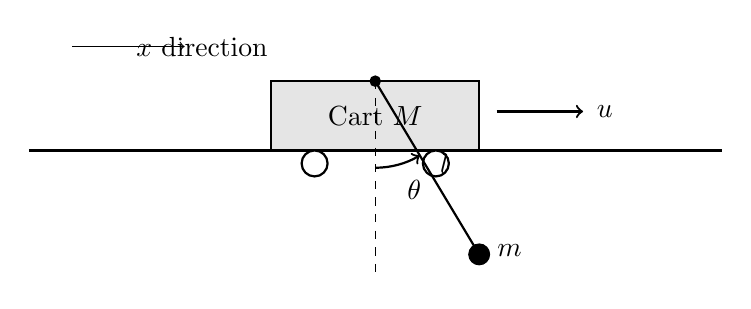
\begin{tikzpicture}[scale=1.1]

    % Ground
    \draw[thick] (-4,0) -- (4,0);

    % Cart
    \draw[fill=gray!20, thick] (-1.2,0) rectangle (1.2,0.8);

    % Wheels
    \draw[thick, fill=white] (-0.7,-0.15) circle (0.15);
    \draw[thick, fill=white] (0.7,-0.15) circle (0.15);

    % Pivot
    \filldraw[black] (0,0.8) circle (0.06);

    % Pendulum rod
    \draw[thick] (0,0.8) -- (1.2,-1.2);

    % Bob
    \filldraw[black] (1.2,-1.2) circle (0.12);

    % Vertical dashed reference
    \draw[dashed] (0,0.8) -- (0,-1.5);

    % Angle arc
    \draw[thick, ->] (0,-0.2) arc[start angle=-90,end angle=-59,radius=1.0];
    \node at (0.45,-0.45) {\(\theta\)};

    % Force arrow
    \draw[->, thick] (1.4,0.45) -- (2.4,0.45);
    \node at (2.65,0.45) {\(u\)};

    % Labels
    \node at (0,0.4) {Cart \(M\)};
    \node at (1.55,-1.15) {\(m\)};
    \node at (0.8,-0.15) {\(l\)};

    % x axis arrow
    \draw[->] (-3.5,1.2) -- (-2.2,1.2);
    \node at (-2.0,1.2) {\(x\) direction};

\end{tikzpicture}
\caption{Cart--pendulum system with angle \(\theta\) measured from the downward vertical.}
\end{figure}

\section{Generalized Coordinates}

We choose the generalized coordinates:
\[
q = \begin{bmatrix} p \\ \theta \end{bmatrix},
\]
where:
\begin{itemize}[leftmargin=2em]
    \item \(p\): horizontal position of the cart,
    \item \(\theta\): pendulum angle measured from the downward vertical.
\end{itemize}

The state vector is:
\[
x = \begin{bmatrix}
p \\ \dot p \\ \theta \\ \dot \theta
\end{bmatrix}.
\]

\section{Kinematics}

The cart position is simply:
\[
x_c = p.
\]

The pendulum bob position is:
\[
x_p = p + l\sin\theta,
\qquad
y_p = -l\cos\theta.
\]

Differentiating:
\[
\dot x_p = \dot p + l\dot\theta\cos\theta,
\qquad
\dot y_p = l\dot\theta\sin\theta.
\]

Hence the bob speed squared is:
\begin{align*}
v_p^2
&= \dot x_p^2 + \dot y_p^2 \\
&= \left(\dot p + l\dot\theta\cos\theta\right)^2
   + \left(l\dot\theta\sin\theta\right)^2 \\
&= \dot p^2 + 2l\dot p\dot\theta\cos\theta + l^2\dot\theta^2.
\end{align*}

\section{Energy of the System}

\subsection{Kinetic Energy}

The kinetic energy of the cart is:
\[
T_c = \frac{1}{2}M\dot p^2.
\]

The kinetic energy of the pendulum bob is:
\[
T_p = \frac{1}{2}m v_p^2
= \frac{1}{2}m\left(\dot p^2 + 2l\dot p\dot\theta\cos\theta + l^2\dot\theta^2\right).
\]

Therefore total kinetic energy is:
\begin{align*}
T &= T_c + T_p \\
&= \frac{1}{2}(M+m)\dot p^2 + ml\dot p\dot\theta\cos\theta + \frac{1}{2}ml^2\dot\theta^2.
\end{align*}

\subsection{Potential Energy}

Taking zero potential at the pivot height reference is not necessary; only differences matter. Since the bob height is
\[
y_p = -l\cos\theta,
\]
the gravitational potential may be written as
\[
V = -mgl\cos\theta.
\]

Thus the downward configuration \(\theta=0\) is a minimum of potential energy.

\section{Lagrangian and Equations of Motion}

The Lagrangian is:
\[
\mathcal{L} = T - V.
\]

So:
\[
\mathcal{L}
=
\frac{1}{2}(M+m)\dot p^2
+ ml\dot p\dot\theta\cos\theta
+ \frac{1}{2}ml^2\dot\theta^2
+ mgl\cos\theta.
\]

We apply the Euler--Lagrange equations with generalized forces:
\[
Q_p = u,
\qquad
Q_\theta = 0.
\]

\subsection{Equation for \(p\)}

First compute:
\[
\frac{\partial \mathcal{L}}{\partial \dot p}
=
(M+m)\dot p + ml\dot\theta\cos\theta.
\]

Then:
\[
\frac{d}{dt}\left(\frac{\partial \mathcal{L}}{\partial \dot p}\right)
=
(M+m)\ddot p
+ ml\ddot\theta\cos\theta
- ml\dot\theta^2\sin\theta.
\]

Also:
\[
\frac{\partial \mathcal{L}}{\partial p} = 0.
\]

Therefore:
\[
(M+m)\ddot p + ml\ddot\theta\cos\theta - ml\dot\theta^2\sin\theta = u.
\]

\subsection{Equation for \(\theta\)}

Now compute:
\[
\frac{\partial \mathcal{L}}{\partial \dot\theta}
=
ml\dot p\cos\theta + ml^2\dot\theta.
\]

Differentiating:
\[
\frac{d}{dt}\left(\frac{\partial \mathcal{L}}{\partial \dot\theta}\right)
=
ml\ddot p\cos\theta
- ml\dot p\dot\theta\sin\theta
+ ml^2\ddot\theta.
\]

Next:
\[
\frac{\partial \mathcal{L}}{\partial \theta}
=
-ml\dot p\dot\theta\sin\theta - mgl\sin\theta.
\]

Thus the Euler--Lagrange equation gives:
\begin{align*}
&ml\ddot p\cos\theta
- ml\dot p\dot\theta\sin\theta
+ ml^2\ddot\theta
- \left(-ml\dot p\dot\theta\sin\theta - mgl\sin\theta\right)
= 0.
\end{align*}

The middle terms cancel, yielding:
\[
ml\ddot p\cos\theta + ml^2\ddot\theta + mgl\sin\theta = 0.
\]

Dividing by \(ml\):
\[
\ddot p\cos\theta + l\ddot\theta + g\sin\theta = 0.
\]

\section{Nonlinear Equations of Motion}

The equations of motion are therefore:
\begin{equation}
(M+m)\ddot p + ml\cos\theta\,\ddot\theta - ml\sin\theta\,\dot\theta^2 = u,
\label{eq:eom1}
\end{equation}
\begin{equation}
\ddot p\cos\theta + l\ddot\theta + g\sin\theta = 0.
\label{eq:eom2}
\end{equation}

\section{Solving for Accelerations}

From \eqref{eq:eom2},
\[
l\ddot\theta = -\ddot p\cos\theta - g\sin\theta,
\]
so
\[
\ddot\theta = -\frac{\cos\theta}{l}\ddot p - \frac{g}{l}\sin\theta.
\]

Substitute this into \eqref{eq:eom1}:
\[
(M+m)\ddot p + ml\cos\theta
\left(
-\frac{\cos\theta}{l}\ddot p - \frac{g}{l}\sin\theta
\right)
- ml\sin\theta\,\dot\theta^2 = u.
\]

Simplifying:
\[
(M+m)\ddot p - m\cos^2\theta\,\ddot p - mg\sin\theta\cos\theta - ml\sin\theta\,\dot\theta^2 = u.
\]

Hence:
\[
\left(M + m - m\cos^2\theta\right)\ddot p
=
u + mg\sin\theta\cos\theta + ml\sin\theta\,\dot\theta^2.
\]

Using
\[
M + m - m\cos^2\theta = M + m\sin^2\theta,
\]
we obtain:
\begin{equation}
\ddot p =
\frac{
u + mg\sin\theta\cos\theta + ml\sin\theta\,\dot\theta^2
}{
M + m\sin^2\theta
}.
\label{eq:ddotp}
\end{equation}

Then:
\begin{equation}
\ddot\theta
=
-\frac{\cos\theta}{l}\ddot p - \frac{g}{l}\sin\theta.
\label{eq:ddottheta}
\end{equation}

Substituting \eqref{eq:ddotp} into \eqref{eq:ddottheta} gives the complete nonlinear dynamics.

\section{State-Space Form}

Define the state:
\[
x =
\begin{bmatrix}
x_1 \\ x_2 \\ x_3 \\ x_4
\end{bmatrix}
=
\begin{bmatrix}
p \\ \dot p \\ \theta \\ \dot\theta
\end{bmatrix}.
\]

Then:
\[
\dot x_1 = x_2,
\qquad
\dot x_3 = x_4.
\]

Using \eqref{eq:ddotp}:
\[
\dot x_2
=
\frac{
u + mg\sin x_3\cos x_3 + ml\sin x_3\,x_4^2
}{
M + m\sin^2 x_3
}.
\]

Using \eqref{eq:ddottheta}:
\[
\dot x_4
=
-\frac{\cos x_3}{l}
\cdot
\frac{
u + mg\sin x_3\cos x_3 + ml\sin x_3\,x_4^2
}{
M + m\sin^2 x_3
}
-\frac{g}{l}\sin x_3.
\]

Thus the system has the control-affine form:
\[
\dot x = f(x) + g(x)u,
\]
where
\[
f(x)=
\begin{bmatrix}
x_2 \\[1ex]
\dfrac{
mg\sin x_3\cos x_3 + ml\sin x_3\,x_4^2
}{
M + m\sin^2 x_3
} \\[3ex]
x_4 \\[1ex]
-\dfrac{\cos x_3}{l}
\dfrac{
mg\sin x_3\cos x_3 + ml\sin x_3\,x_4^2
}{
M + m\sin^2 x_3
}
-\dfrac{g}{l}\sin x_3
\end{bmatrix}
\]
and
\[
g(x)=
\begin{bmatrix}
0 \\[1ex]
\dfrac{1}{M + m\sin^2 x_3} \\[3ex]
0 \\[1ex]
-\dfrac{\cos x_3}{l\left(M + m\sin^2 x_3\right)}
\end{bmatrix}.
\]

\section{Equilibrium Point}

We want the cart to settle at a desired position \(B\) while the pendulum hangs downward. The desired equilibrium is:
\[
x^\star =
\begin{bmatrix}
B \\ 0 \\ 0 \\ 0
\end{bmatrix}.
\]

Define the regulation error:
\[
e = x - x^\star =
\begin{bmatrix}
p-B \\ \dot p \\ \theta \\ \dot\theta
\end{bmatrix}.
\]

\section{Linearization Around the Downward Equilibrium}

Assume small angles:
\[
\sin\theta \approx \theta,
\qquad
\cos\theta \approx 1,
\qquad
\theta\dot\theta^2 \approx 0.
\]

Then:
\[
\ddot p \approx \frac{u + mg\theta}{M},
\]
and
\[
\ddot\theta \approx -\frac{1}{l}\ddot p - \frac{g}{l}\theta.
\]

Substituting \(\ddot p\):
\[
\ddot\theta \approx -\frac{1}{Ml}u - \frac{(M+m)g}{Ml}\theta.
\]

Therefore the linearized dynamics are:
\[
\dot e = Ae + Bu,
\]
with
\[
A =
\begin{bmatrix}
0 & 1 & 0 & 0 \\
0 & 0 & \dfrac{mg}{M} & 0 \\
0 & 0 & 0 & 1 \\
0 & 0 & -\dfrac{(M+m)g}{Ml} & 0
\end{bmatrix},
\qquad
B =
\begin{bmatrix}
0 \\[1ex]
\dfrac{1}{M} \\[1ex]
0 \\[1ex]
-\dfrac{1}{Ml}
\end{bmatrix}.
\]

\section{Approach 3: CLF/CCM-Inspired QP Control}

\subsection{Step 1: Choose a Nominal Controller}

A nominal controller is chosen first, typically from LQR:
\[
u_{\mathrm{nom}} = -Ke,
\]
where \(K\) is designed from the linearized system.

This nominal control attempts to regulate:
\begin{itemize}[leftmargin=2em]
    \item cart position \(p \to B\),
    \item cart velocity \(\dot p \to 0\),
    \item pendulum angle \(\theta \to 0\),
    \item angular velocity \(\dot\theta \to 0\).
\end{itemize}

\noindent\textbf{MATLAB implementation} (\texttt{script\_10a}, Part~A): An LQR controller is designed at the linearization point \(x=0\):

\begin{lstlisting}
Q_lqr = diag([10, 1, 50, 1]);   R_lqr = 1;
[K_lqr, P_lqr, ~] = lqr(A0, B0, Q_lqr, R_lqr);
\end{lstlisting}

\begin{codemath}
The code computes a linear quadratic regulator for the linearized error dynamics
\[
\dot e = A_0\, e + B_0\, u,
\]
minimizing the infinite-horizon cost
\[
J = \int_0^\infty \bigl( e^\top Q_{\mathrm{lqr}}\, e + R_{\mathrm{lqr}}\, u^2 \bigr)\,dt,
\qquad
Q_{\mathrm{lqr}} = \operatorname{diag}(10,\,1,\,50,\,1),
\quad
R_{\mathrm{lqr}} = 1.
\]
MATLAB's \texttt{lqr} solves the continuous algebraic Riccati equation
\[
A_0^\top P + P A_0 - P B_0\, R_{\mathrm{lqr}}^{-1} B_0^\top P + Q_{\mathrm{lqr}} = 0,
\]
and returns the optimal gain
\[
K_{\mathrm{lqr}} = R_{\mathrm{lqr}}^{-1}\, B_0^\top P.
\]
The nominal stabilizing feedback law is therefore
\[
u_{\mathrm{nom}} = -K_{\mathrm{lqr}}\, e.
\]
The Riccati matrix \(P\) is reused as the \emph{constant} CLF metric in subsequent controllers.
\end{codemath}

\subsection{Step 2: Define the CLF / Energy Function}

Choose a positive definite matrix \(P=P^\top>0\), for example from the algebraic Riccati equation used in LQR, and define
\[
V(e) = e^\top P e.
\]

This is the Control Lyapunov Function (CLF), or equivalently a contraction-inspired quadratic energy.

\subsection{Step 3: Differentiate the CLF}

Since
\[
V(e)=e^\top P e,
\]
its derivative is
\[
\dot V = 2e^\top P \dot e.
\]

For a constant target \(x^\star\), we have
\[
\dot e = \dot x = f(x)+g(x)u.
\]

Hence:
\[
\dot V = 2e^\top P\bigl(f(x)+g(x)u\bigr).
\]

Define:
\[
a(x) = 2e^\top P f(x),
\qquad
b(x) = 2e^\top P g(x).
\]

Then:
\[
\dot V = a(x) + b(x)u.
\]

\subsection{Step 4: Impose Exponential Decay}

To ensure stability, impose:
\[
\dot V \le -2\lambda V,
\qquad \lambda > 0.
\]

Substituting the expression for \(\dot V\):
\[
a(x)+b(x)u \le -2\lambda V(x).
\]

This inequality constrains the control input.

\subsection{Step 5: Solve the Minimum-Norm QP}

The actual control is chosen as the solution of:
\[
\min_u \frac{1}{2}(u-u_{\mathrm{nom}})^2
\]
subject to
\[
a(x)+b(x)u \le -2\lambda V(x).
\]

This means:
\begin{itemize}[leftmargin=2em]
    \item stay as close as possible to the nominal control,
    \item but modify it when needed to guarantee Lyapunov decrease.
\end{itemize}

\subsection{Step 6: Closed-Form Solution}

Define
\[
c(x) = -2\lambda V(x) - a(x).
\]

Then the constraint becomes:
\[
b(x)u \le c(x).
\]

Because \(u\) is scalar, the QP has a simple solution:

\[
u =
\begin{cases}
u_{\mathrm{nom}}, & \text{if } b(x)u_{\mathrm{nom}} \le c(x), \\[1.2ex]
\dfrac{c(x)}{b(x)}, & \text{if } b(x)u_{\mathrm{nom}} > c(x)\text{ and } b(x)\neq 0.
\end{cases}
\]

In practice, if \(b(x)\) is very small, one typically:
\begin{itemize}[leftmargin=2em]
    \item uses \(u_{\mathrm{nom}}\), or
    \item adds a slack variable to guarantee numerical robustness.
\end{itemize}

\noindent\textbf{MATLAB implementation} (\texttt{script\_10a}, Part~D):

\begin{lstlisting}
function u = clf_qp_controller(x, x_star, f_fn, B_fn, K_lqr, P, lam)
    e = x - x_star;
    u_nom = -K_lqr * e;
    V     = e' * P * e;               % CLF
    a_val = 2 * e' * P * f_fn(x);     % Vdot unforced part
    b_val = 2 * e' * P * B_fn(x);     % Vdot control coefficient
    c_val = -2*lam*V - a_val;          % constraint RHS
    if b_val * u_nom <= c_val
        u = u_nom;                     % nominal already satisfies
    elseif abs(b_val) > 1e-10
        u = c_val / b_val;            % project onto constraint
    else
        u = u_nom;
    end
end
\end{lstlisting}

\begin{codemath}
The function implements the scalar CLF-QP controller. Given the error \(e = x - x^\star\), the quantities
\[
V = e^\top P\, e, \qquad
a(x) = 2\,e^\top P\, f(x), \qquad
b(x) = 2\,e^\top P\, B(x)
\]
are evaluated, so that \(\dot V = a(x) + b(x)\,u\). The exponential decay constraint \(\dot V \le -2\lambda V\) is rewritten as \(b(x)\,u \le c(x)\) with
\[
c(x) = -2\lambda\, V - a(x).
\]
The closed-form solution of the one-dimensional QP is:
\[
u =
\begin{cases}
u_{\mathrm{nom}}, & \text{if } b(x)\,u_{\mathrm{nom}} \le c(x), \\[1ex]
\dfrac{c(x)}{b(x)}, & \text{if } b(x)\,u_{\mathrm{nom}} > c(x) \text{ and } |b(x)| > \epsilon, \\[1.5ex]
u_{\mathrm{nom}}, & \text{if } |b(x)| \le \epsilon \quad (\text{singularity guard}).
\end{cases}
\]
No numerical optimizer is invoked; the entire controller reduces to one branch evaluation per time step.
\end{codemath}

Because the constraint is a single scalar inequality and \(u\) is scalar, the QP has a closed-form solution (no solver needed).  Online cost: one evaluation of \(f(x)\), \(B(x)\), and a matrix-vector product \(Pe\).

\section{Interpretation of the Controller}

This controller works in two layers:

\begin{enumerate}[leftmargin=2em]
    \item The \textbf{nominal controller} gives the desired motion toward the target.
    \item The \textbf{QP layer} corrects the nominal input only when necessary to ensure decay of the total energy \(V\).
\end{enumerate}

Thus the controller simultaneously:
\begin{itemize}[leftmargin=2em]
    \item drives the cart to the target position,
    \item damps pendulum oscillation,
    \item preserves stability in a systematic optimization-based way.
\end{itemize}

\section{Trajectory Tracking Version}

If instead of regulating directly to \(B\), we want the cart to follow a smooth reference trajectory \(p_r(t)\), define
\[
x_r(t)=
\begin{bmatrix}
p_r(t) \\ \dot p_r(t) \\ 0 \\ 0
\end{bmatrix},
\qquad
e = x - x_r(t).
\]

Then:
\[
\dot e = f(x)+g(x)u - \dot x_r.
\]

The CLF derivative becomes:
\[
\dot V = 2e^\top P\bigl(f(x)+g(x)u-\dot x_r\bigr).
\]

Define:
\[
a(x,t)=2e^\top P\bigl(f(x)-\dot x_r\bigr),
\qquad
b(x,t)=2e^\top P g(x).
\]

Then solve:
\[
\min_u \frac{1}{2}(u-u_{\mathrm{nom}})^2
\]
subject to
\[
a(x,t)+b(x,t)u \le -2\lambda V.
\]

This trajectory-tracking formulation is often preferable for moving from \(A\) to \(B\), since it avoids abrupt commands.

\section{Limitations of Approach~3 (CLF-QP with Constant \(P\))}

While Approach~3 is intuitive and computationally cheap, it has important limitations when compared with the full CCM framework of Manchester \& Slotine (2017):

\begin{enumerate}[leftmargin=2em]
    \item \textbf{Constant metric:} The matrix \(P\) from LQR is constant (state-independent). It only certifies stability locally near the linearization point.
    \item \textbf{No CCM feasibility verification:} The dual CCM condition (eq.~11 of the paper) is never checked globally.
    \item \textbf{No geodesic computation:} The paper's controller integrates along geodesics in the state-dependent metric. Approach~3 implicitly uses straight lines, which are geodesics only for constant metrics.
    \item \textbf{No universal stabilizability guarantee:} The paper guarantees exponential convergence from \emph{any} initial condition. Approach~3 only guarantees local stability where the LQR linearization is valid.
\end{enumerate}

\section{Full CCM Implementation (Manchester \& Slotine, 2017)}

We now present the full CCM-based controller for the cart--pendulum, following \cite{manchester2017ccm}.

\subsection{Step 1: System in Control-Affine Form}

The cart--pendulum is already in control-affine form:
\[
\dot x = f(x) + B(x)\,u,
\]
with state \(x = [p,\; \dot p,\; \theta,\; \dot\theta]^\top\) and single input \(u\) (cart force).

\noindent\textbf{MATLAB implementation} (\texttt{script\_10a}, Part~A): The exact nonlinear model (no linearization) with denominator \(D(\theta) = M_c + m_p\sin^2\theta\):

\begin{lstlisting}
f_fn = @(x) [ ...
    x(2); ...
    (mp*g*sin(x(3))*cos(x(3)) + mp*lp*sin(x(3))*x(4)^2) ...
        / (Mc + mp*sin(x(3))^2); ...
    x(4); ...
    -(cos(x(3))/lp) * (mp*g*sin(x(3))*cos(x(3)) ...
        + mp*lp*sin(x(3))*x(4)^2) ...
        / (Mc + mp*sin(x(3))^2) - (g/lp)*sin(x(3)) ];

B_fn = @(x) [ 0;
    1/(Mc + mp*sin(x(3))^2);
    0;
    -cos(x(3)) / (lp*(Mc + mp*sin(x(3))^2)) ];
\end{lstlisting}

\begin{codemath}
Defining \(D(\theta) = M_c + m_p\sin^2\theta\), the drift vector field is
\[
f(x)=
\begin{bmatrix}
x_2 \\[1ex]
\dfrac{m_p g \sin x_3 \cos x_3 + m_p l_p \sin x_3\, x_4^2}{D(x_3)} \\[3ex]
x_4 \\[1ex]
-\dfrac{\cos x_3}{l_p}
\cdot
\dfrac{m_p g \sin x_3 \cos x_3 + m_p l_p \sin x_3\, x_4^2}{D(x_3)}
-\dfrac{g}{l_p}\sin x_3
\end{bmatrix},
\]
and the input vector field is
\[
B(x)=
\begin{bmatrix}
0 \\[1ex]
\dfrac{1}{D(x_3)} \\[3ex]
0 \\[1ex]
-\dfrac{\cos x_3}{l_p\,D(x_3)}
\end{bmatrix}.
\]
The control input \(u\) acts directly on cart acceleration and indirectly (through inertial coupling) on pendulum angular acceleration.
\end{codemath}

The Jacobian \(A(x) = \partial f/\partial x\) is computed via forward-difference numerical differentiation, avoiding lengthy symbolic expressions:

\begin{lstlisting}
function J = numjac4(f_fn, x)
    n = 4;  h = 1e-7;
    f0 = f_fn(x);
    J = zeros(n, n);
    for i = 1:n
        xp = x; xp(i) = xp(i) + h;
        J(:,i) = (f_fn(xp) - f0) / h;
    end
end
\end{lstlisting}

\begin{codemath}
The function approximates the Jacobian \(A(x) = \partial f/\partial x\) using first-order forward differences. The \(i\)-th column is
\[
A_{:,\,i}(x) \approx \frac{f(x + h\, e_i) - f(x)}{h},
\qquad h = 10^{-7},
\]
where \(e_i\) is the \(i\)-th standard basis vector. The assembled Jacobian is
\[
A(x) \approx
\begin{bmatrix}
\dfrac{f(x+h e_1)-f(x)}{h} &
\dfrac{f(x+h e_2)-f(x)}{h} &
\dfrac{f(x+h e_3)-f(x)}{h} &
\dfrac{f(x+h e_4)-f(x)}{h}
\end{bmatrix}.
\]
This Jacobian enters the CCM dual condition through the symmetrized product \(A(x)\,W + W\,A(x)^\top\).
\end{codemath}

\subsection{Step 2: Dual CCM Condition}

We search for a \textbf{state-dependent dual metric} \(W(x) = M(x)^{-1} \succ 0\) satisfying the convex condition (eq.~11 of the paper):
\begin{equation}
-\frac{\partial W}{\partial t} - \partial_f W + \frac{\partial f}{\partial x}W + W\frac{\partial f^\top}{\partial x} - \rho B B^\top + 2\lambda W \prec 0
\label{eq:ccm_dual}
\end{equation}
for all \(x\) in the region of interest, where:
\begin{itemize}[leftmargin=2em]
    \item \(\partial_f W = \sum_j \frac{\partial W}{\partial x_j} f_j(x)\) is the Lie derivative of \(W\) along \(f\),
    \item \(\rho(x) > 0\) is a scalar multiplier (decision variable),
    \item \(\lambda > 0\) is the desired contraction rate.
\end{itemize}

This is \textbf{jointly convex} in \(W\) and \(\rho\), and can be solved via SDP on a grid or via SOS programming.

For a time-invariant system, \(\partial W/\partial t = 0\), so condition \eqref{eq:ccm_dual} simplifies to:
\begin{equation}
-\partial_f W + \frac{\partial f}{\partial x}W + W\frac{\partial f^\top}{\partial x} - \rho B B^\top + 2\lambda W \prec 0.
\label{eq:ccm_dual_ti}
\end{equation}

\subsection{Step 3: Parameterize \(W(x)\) and \(\rho(x)\)}

We parameterize \(W(x)\) as a polynomial (e.g.\ quadratic) function of the state:
\[
W(x) = W_0 + \sum_i W_i\, x_i + \sum_{i \le j} W_{ij}\, x_i x_j,
\]
where \(W_0, W_i, W_{ij}\) are symmetric \(4\times 4\) decision matrices.

The multiplier \(\rho(x)\) can also be polynomial. In the simplest case, \(\rho\) is a positive constant.

The constraints are enforced at grid points \(x^{(k)}\) in a box \(\mathcal{D}\):
\[
W(x^{(k)}) \succeq \varepsilon_W I, \qquad
\Sigma(x^{(k)}) \preceq -\varepsilon_S I,
\]
where \(\Sigma\) is the left-hand side of \eqref{eq:ccm_dual_ti}. This yields a finite-dimensional SDP solvable with YALMIP + SeDuMi.

\noindent\textbf{MATLAB implementation} (\texttt{script\_10a}, Part~B): The dual metric is parameterized as a \textbf{quadratic polynomial} in \((\theta, \dot\theta)\).  Each coefficient is a symmetric \(4\times 4\) YALMIP decision matrix (\(6 \times 10 = 60\) scalar unknowns):

\begin{lstlisting}
W0      = sdpvar(4, 4, 'symmetric');   % constant term
W_th    = sdpvar(4, 4, 'symmetric');   % theta coefficient
W_thd   = sdpvar(4, 4, 'symmetric');   % theta_dot coefficient
W_th2   = sdpvar(4, 4, 'symmetric');   % theta^2 coefficient
W_ththd = sdpvar(4, 4, 'symmetric');   % theta*theta_dot coefficient
W_thd2  = sdpvar(4, 4, 'symmetric');   % theta_dot^2 coefficient

rho0 = sdpvar(1);  rho1 = sdpvar(1);  % rho = rho0 + rho1*theta^2
\end{lstlisting}

\begin{codemath}
The dual metric is parameterized as a quadratic polynomial in \(\theta\) and \(\dot\theta\):
\[
W(\theta,\dot\theta)
=
W_0
+ W_\theta\,\theta
+ W_{\dot\theta}\,\dot\theta
+ W_{\theta^2}\,\theta^2
+ W_{\theta\dot\theta}\,\theta\,\dot\theta
+ W_{\dot\theta^2}\,\dot\theta^2,
\]
where each coefficient \(W_0, W_\theta, \ldots, W_{\dot\theta^2}\) is a symmetric \(4\times 4\) decision matrix.

The scalar multiplier is parameterized as
\[
\rho(\theta) = \rho_0 + \rho_1\,\theta^2.
\]
\(W\) does not depend on \(p\) (translation-invariant dynamics) or \(\dot p\) (for tractability), keeping the SDP small while allowing state-dependent adaptation in the pendulum coordinates.
\end{codemath}

The Lie derivative \(\partial_f W\) is computed analytically from the polynomial structure:

\begin{lstlisting}
dWdth  = W_th + 2*W_th2*x3k + W_ththd*x4k;       % dW/d(theta)
dWdthd = W_thd + W_ththd*x3k + 2*W_thd2*x4k;     % dW/d(theta_dot)
Wdot_k = dWdth * fk(3) + dWdthd * fk(4);          % chain rule
\end{lstlisting}

\begin{codemath}
The partial derivatives of the polynomial metric are
\[
\frac{\partial W}{\partial \theta}
=
W_\theta + 2\,W_{\theta^2}\,\theta + W_{\theta\dot\theta}\,\dot\theta,
\qquad
\frac{\partial W}{\partial \dot\theta}
=
W_{\dot\theta} + W_{\theta\dot\theta}\,\theta + 2\,W_{\dot\theta^2}\,\dot\theta.
\]
By the chain rule, the Lie derivative of \(W\) along the drift \(f(x)\) is
\[
\partial_f W
=
\frac{\partial W}{\partial \theta}\,f_3(x)
+
\frac{\partial W}{\partial \dot\theta}\,f_4(x),
\]
where \(f_3 = \dot\theta\) and \(f_4 = \ddot\theta_{\text{unforced}}\). At a grid point \(x^{(k)}\) this becomes
\[
\texttt{Wdot\_k}
=
\left.\frac{\partial W}{\partial \theta}\right|_{x^{(k)}}\! f_3(x^{(k)})
\;+\;
\left.\frac{\partial W}{\partial \dot\theta}\right|_{x^{(k)}}\! f_4(x^{(k)}).
\]
\end{codemath}

At each grid point \(x^{(k)}\), the constraint matrix \(\Sigma\) from eq.~\eqref{eq:ccm_dual_ti} is assembled:

\begin{lstlisting}
Sigma_k = -Wdot_k + Ak*Wk + Wk*Ak' ...
           - rhok*(Bk*Bk') + 2*lambda_ccm*Wk;
\end{lstlisting}

\begin{codemath}
This is \textbf{exactly} the left-hand side of the dual CCM condition~\eqref{eq:ccm_dual_ti}, with a one-to-one code--equation correspondence:
\[
\Sigma
= \underbrace{-\partial_f W\vphantom{\frac{\partial f}{\partial x}}}_{-\,\texttt{Wdot\_k}}
+ \underbrace{\frac{\partial f}{\partial x}W + W\frac{\partial f^\top}{\partial x}}_{\texttt{Ak*Wk\;+\;Wk*Ak'}}
- \underbrace{\rho\, B B^\top\vphantom{\frac{\partial f}{\partial x}}}_{\texttt{rhok*(Bk*Bk')}}
+ \underbrace{2\lambda\, W\vphantom{\frac{\partial f}{\partial x}}}_{\texttt{2*lambda\_ccm*Wk}}.
\]
Since \(A_k, B_k\) are \emph{numeric} at each grid point while \(W_k, \rho_k\) remain \emph{sdpvar} expressions, \(\Sigma_k\) is \textbf{linear} in the decision variables---hence the problem is a convex SDP.
\end{codemath}

Two LMIs are imposed at each of the \(N^3\) grid points:

\begin{lstlisting}
F_ccm = [F_ccm, -Sigma_k - epsS*eye(4) >= 0];  % Sigma < -epsS*I
F_ccm = [F_ccm,  Wk      - epsW*eye(4) >= 0];  % W     >  epsW*I
\end{lstlisting}

\begin{codemath}
These two matrix inequalities enforce strict feasibility with numerical margins:
\[
-\Sigma_k - \varepsilon_S\, I \succeq 0
\quad\Longleftrightarrow\quad
\Sigma_k \preceq -\varepsilon_S\, I
\qquad\text{(contraction)},
\]
\[
W_k - \varepsilon_W\, I \succeq 0
\quad\Longleftrightarrow\quad
W_k \succeq \varepsilon_W\, I
\qquad\text{(positive definiteness)}.
\]
The second condition ensures that \(W(x)\) is uniformly bounded away from singularity, so the primal metric \(M(x) = W(x)^{-1}\) remains well defined.
\end{codemath}

The SDP is solved as a \emph{feasibility} problem (no objective):

\begin{lstlisting}
opts_sdp = sdpsettings('verbose', 1, 'solver', 'sedumi');
sol_ccm  = optimize(F_ccm, [], opts_sdp);
\end{lstlisting}

\begin{codemath}
The call solves a semidefinite feasibility problem:
\[
\text{find}\quad
\bigl\{W_0,\,W_\theta,\,W_{\dot\theta},\,W_{\theta^2},\,W_{\theta\dot\theta},\,W_{\dot\theta^2},\,\rho_0,\,\rho_1\bigr\}
\]
subject to
\[
W\!\bigl(x^{(k)}\bigr) \succeq \varepsilon_W\, I,
\qquad
\Sigma\!\bigl(x^{(k)}\bigr) \preceq -\varepsilon_S\, I,
\qquad
\rho_0 > 0,
\]
for every grid point \(x^{(k)} \in \mathcal{D}\). No objective is minimized; the problem determines whether a feasible contraction metric exists within the parameterized family.
\end{codemath}

\textbf{Complexity:} With a \(5^3 = 125\) grid, there are \(250\) matrix constraints of size \(4 \times 4\) plus 2 scalar constraints on \(\rho\) -- a modest SDP solvable in under a second.  If infeasible, the script retries with a smaller \(\lambda\).

\subsection{Step 4: Differential Feedback Gain}

Once \(W(x)\) and \(\rho(x)\) are found, the differential feedback gain is:
\[
K(x) = -\tfrac{1}{2}\,\rho(x)\,B(x)^\top W(x)^{-1} = -\tfrac{1}{2}\,\rho(x)\,B(x)^\top M(x).
\]

This satisfies the closed-loop contraction condition:
\[
\dot M + \bigl(A + BK\bigr)^\top M + M\bigl(A + BK\bigr) + 2\lambda M \prec 0.
\]

\noindent\textbf{MATLAB implementation} (\texttt{script\_10a}, Part~C): After the SDP solve, numeric matrices are extracted and the metric is constructed using a robust regularized inverse:

\begin{lstlisting}
W0v     = value(W0);     W_thv   = value(W_th);   ...
rho0v   = value(rho0);   rho1v   = value(rho1);

W_num = @(th, thd) W0v + W_thv*th + W_thdv*thd ...
    + W_th2v*th^2 + W_ththdv*th*thd + W_thd2v*thd^2;
M_num = @(th, thd) robust_W_inv(W_num(th, thd));
\end{lstlisting}

\begin{codemath}
After the SDP solver returns, symbolic decision variables are extracted as numeric matrices. The dual metric evaluator is
\[
W(\theta,\dot\theta)
=
W_0^{(v)} + W_\theta^{(v)}\,\theta + W_{\dot\theta}^{(v)}\,\dot\theta
+ W_{\theta^2}^{(v)}\,\theta^2
+ W_{\theta\dot\theta}^{(v)}\,\theta\,\dot\theta
+ W_{\dot\theta^2}^{(v)}\,\dot\theta^2,
\]
and the primal (contraction) metric is obtained by regularized inversion:
\[
M(\theta,\dot\theta) = W(\theta,\dot\theta)^{-1}.
\]
The helper \texttt{robust\_W\_inv} symmetrizes \(W\), clamps eigenvalues away from zero via eigendecomposition, and reconstructs \(M\) to prevent numerical blow-up near the boundary of the synthesis region.
\end{codemath}

\subsection{Step 5: Geodesic Computation}

Given the current state \(x(t)\) and target state \(x^\star(t)\), compute the minimal geodesic \(\gamma : [0,1] \to \mathbb{R}^n\) with:
\[
\gamma(0) = x^\star(t), \qquad \gamma(1) = x(t),
\]
minimizing the Riemannian energy:
\[
E(\gamma) = \int_0^1 \gamma_s(s)^\top M(\gamma(s))\,\gamma_s(s)\,ds.
\]

For a \textbf{constant metric} \(M = P\) (state-independent), geodesics are straight lines:
\[
\gamma(s) = x^\star + s\,(x - x^\star), \qquad \gamma_s = x - x^\star.
\]

For a \textbf{state-dependent metric}, geodesics satisfy the geodesic ODE:
\begin{equation}
\ddot\gamma^i + \Gamma^i_{jk}\,\dot\gamma^j\,\dot\gamma^k = 0,
\label{eq:geodesic_ode}
\end{equation}
where the Christoffel symbols of the second kind are:
\begin{equation}
\Gamma^i_{jk} = \frac{1}{2}\sum_l M^{il}\!\left(\frac{\partial M_{lj}}{\partial x_k} + \frac{\partial M_{lk}}{\partial x_j} - \frac{\partial M_{jk}}{\partial x_l}\right),
\label{eq:christoffel}
\end{equation}
with \(M^{il}\) denoting elements of \(M^{-1}\).

\subsubsection{Shooting Method with Levenberg--Marquardt}

We solve the geodesic boundary-value problem via a \textbf{single shooting method}: guess the initial velocity \(v_0 = \dot\gamma(0)\), integrate the geodesic ODE~\eqref{eq:geodesic_ode} from \(s = 0\) to \(s = 1\), and iteratively correct \(v_0\) until the endpoint matches \(x(t)\).

The initial velocity is refined using \textbf{Levenberg--Marquardt} iterations:
\[
\Delta v = -\bigl(J^\top J + \mu I\bigr)^{-1} J^\top e_{\rm bc},
\]
where \(e_{\rm bc} = \gamma(1) - x(t)\) is the boundary condition residual, \(J = \partial\gamma(1)/\partial v_0\) is the shooting Jacobian (computed by finite differences), and \(\mu > 0\) is the damping parameter (adapted between \(10^{-4}\) and \(100\) based on progress). The step size is clamped: \(\|\Delta v\| \le 2\|v_0\|\).

\subsubsection{Continuation Strategy for Long Geodesics}

For large \(\|x - x^\star\|\), direct shooting may fail. We use a \textbf{continuation strategy}: divide the displacement into \(N_{\rm cont}\) stages with \(\alpha_k = k/N_{\rm cont}\), and solve sequentially for intermediate targets \(x^\star + \alpha_k\,(x - x^\star)\), warm-starting each stage from the previous solution scaled by \(\alpha_{k+1}/\alpha_k\).

The number of continuation stages is:
\[
N_{\rm cont} = \begin{cases} 1, & \|x - x^\star\| \le 4, \\ \max(2, \lceil \|x - x^\star\| / 3 \rceil), & \text{otherwise.} \end{cases}
\]

\subsubsection{Warm-Starting and Timeout}

In the simulation loop, the initial velocity from the previous time step is reused as a warm-start hint for the current step, greatly improving convergence for nearby states.  A \textbf{wall-clock timeout} of 1~second prevents the shooting solver from stalling during simulation.  If the solver fails or times out, the controller automatically falls back to the straight-line geodesic approximation.

\subsubsection{Christoffel Symbols Implementation}

The Christoffel symbols~\eqref{eq:christoffel} needed by the geodesic ODE are computed via central finite differences at step size \(h = 10^{-5}\):

\begin{lstlisting}
function Gamma = christoffel_symbols(M, x, M_num)
    n = length(x);
    Minv = robust_inv(M);
    dM = zeros(n,n,n);
    h = 1e-5;
    for k = 1:n
        xph = x; xph(k) = xph(k) + h;
        xmh = x; xmh(k) = xmh(k) - h;
        dM(:,:,k) = (M_num(xph(3),xph(4)) ...
                   - M_num(xmh(3),xmh(4))) / (2*h);
    end
    Gamma = zeros(n,n,n);
    for i = 1:n
        for j = 1:n
            for k = 1:n
                s_l = zeros(n,1);
                for l = 1:n
                    s_l(l) = dM(l,j,k) + dM(l,k,j) - dM(j,k,l);
                end
                Gamma(i,j,k) = 0.5 * Minv(i,:) * s_l;
            end
        end
    end
end
\end{lstlisting}

\begin{codemath}
The Christoffel symbols of the second kind for the Riemannian metric \(M(x)\) are
\[
\Gamma^i_{jk}
=
\frac{1}{2}
\sum_{l=1}^{n}
M^{il}
\left(
\frac{\partial M_{lj}}{\partial x_k}
+
\frac{\partial M_{lk}}{\partial x_j}
-
\frac{\partial M_{jk}}{\partial x_l}
\right),
\]
where \(M^{il}\) denotes the \((i,l)\) entry of \(M^{-1}\). The metric partial derivatives are approximated by central differences:
\[
\frac{\partial M}{\partial x_k}\bigg|_x
\approx
\frac{M(x + h\, e_k) - M(x - h\, e_k)}{2h},
\qquad h = 10^{-5}.
\]
These symbols enter the geodesic ODE
\[
\ddot\gamma^i + \Gamma^i_{jk}(\gamma)\;\dot\gamma^j\,\dot\gamma^k = 0,
\]
which defines the shortest paths (energy-minimizing curves) in the Riemannian geometry induced by the CCM.
\end{codemath}

\subsection{Step 6: Control Law via Path Integration}

The actual control input is obtained by integrating the differential feedback along the geodesic:
\[
u(t) = u^\star(t) + \int_0^1 K(\gamma(s))\,\gamma_s(s)\,ds.
\]

For the regulation case where \(x^\star\) is an equilibrium with \(u^\star = 0\):
\[
u(t) = \int_0^1 K(\gamma(s))\,\gamma_s(s)\,ds
     = -\frac{\rho}{2}\int_0^1 B(\gamma(s))^\top M(\gamma(s))\,\gamma_s(s)\,ds.
\]

When \(M = P\) is constant, this simplifies to:
\[
u = -\frac{\rho}{2}\,B(x)^\top P\,(x - x^\star) \cdot \text{(approx.)},
\]
which recovers a linear-like state feedback.

\noindent\textbf{MATLAB implementation} (\texttt{script\_10a}, Part~D): The controller accepts an abstract geodesic function, allowing both straight-line and numerically computed geodesics:

\begin{lstlisting}
function u = ccm_controller(x, x_star, u_star, geodesic_fn, ...
                            B_fn, M_num, rho_num, Ns)
    s_pts = linspace(0, 1, Ns);   ds = 1/(Ns-1);
    integral_K_ds = 0;
    for k = 1:Ns
        [gamma_s, gamma_ds] = geodesic_fn(s_pts(k));
        B_s   = B_fn(gamma_s);
        M_s   = M_num(gamma_s(3), gamma_s(4));
        rho_s = rho_num(gamma_s(3));
        K_s   = (rho_s / 2) * (B_s' * M_s);
        integrand_k = K_s * gamma_ds;
        w = (k == 1 || k == Ns) * 0.5 ...
          + (k > 1  && k < Ns) * 1.0;   % trapezoidal weights
        integral_K_ds = integral_K_ds + w * integrand_k * ds;
    end
    u = u_star - integral_K_ds;
end
\end{lstlisting}

\begin{codemath}
The CCM path-integral control law is
\[
u(t)
=
u^\star(t) - \int_0^1 K\!\bigl(\gamma(s)\bigr)\;\gamma_s(s)\;ds,
\]
where the differential feedback gain at each point along the geodesic is
\[
K(x) = \frac{\rho(x)}{2}\;B(x)^\top M(x).
\]
Substituting gives
\[
u(t)
=
u^\star(t)
-
\int_0^1
\frac{\rho(\gamma(s))}{2}\;
B\!\bigl(\gamma(s)\bigr)^\top
M\!\bigl(\gamma(s)\bigr)\;
\gamma_s(s)\;ds.
\]
The integral is approximated by the composite trapezoidal rule on \(N_s\) nodes:
\[
\int_0^1 \phi(s)\,ds
\;\approx\;
\Delta s\;\sum_{k=1}^{N_s} w_k\;\phi(s_k),
\qquad
w_1 = w_{N_s} = \tfrac{1}{2},
\quad
w_k = 1 \;\text{ for } 2 \le k \le N_s - 1.
\]
\end{codemath}

Two geodesic ``factory'' functions produce the \texttt{geodesic\_fn} closure:
\begin{itemize}[leftmargin=2em]
\item \textbf{Straight-line} (\texttt{geodesic\_straight\_line}): \(\gamma(s) = x^\star + s(x - x^\star)\). Exact for constant \(M\); approximation otherwise.
\item \textbf{Numeric} (\texttt{geodesic\_numeric}): Solves the geodesic BVP via shooting (Step~5). Falls back to straight-line on failure or timeout.
\end{itemize}

\noindent The script runs four controllers for comparison: (1)~LQR, (2)~CLF-QP, (3)~CCM straight-line, (4)~CCM geodesic.  Controller~4 warm-starts the shooting solver using the previous time step's \(v_0\).  Once \(W(x)\) and \(\rho(x)\) are found offline, the path-integral controller requires no online optimization.

\subsection{Step 7: CLF Interpretation and Riemannian Energy}

The Riemannian energy \(E(x, x^\star) = d(x, x^\star)^2\) serves as a CLF:
\[
\frac{d}{dt}E(x, x^\star, t) \le -2\lambda\, E(x, x^\star, t).
\]

From the paper's eq.~12 (first variation of energy):
\[
\frac{1}{2}\frac{d}{dt}E = \langle \gamma_s(0),\, \dot x^\star \rangle_{x^\star} - \langle \gamma_s(1),\, f(x)\rangle_{x} - \langle \gamma_s(1),\, B(x)\,u\rangle_{x} + \frac{1}{2}\frac{\partial E}{\partial t},
\]
which is \textbf{affine in \(u\)}. The set
\[
\mathcal{U} = \left\{ u \in \mathbb{R}^m : \frac{d}{dt}E \le -2\lambda E \right\}
\]
is always nonempty (guaranteed by CCM existence). One can then use pointwise min-norm control:
\[
u(t) = \arg\min_{\tilde u \in \mathcal{U}} \|\tilde u\|^2.
\]

\subsection{Summary: Approach~3 vs Full CCM}

\begin{center}
\begin{tabular}{>{\raggedright}p{4.5cm} p{4.5cm} p{4.5cm}}
\toprule
\textbf{Aspect} & \textbf{Approach 3 (CLF-QP)} & \textbf{Full CCM (Paper)} \\
\midrule
Metric & Constant \(P\) (LQR) & State-dep.\ \(M(x)\) via SDP \\
CLF & \(V = e^\top P e\) & Riemannian energy \(E = d(x,x^\star)^2\) \\
Geodesic & Straight line (implicit) & Shooting method (LM + continuation) \\
Controller & QP: project \(u_{\rm nom}\) & Path integral of \(K(\gamma(s))\gamma_s\) \\
Stability & Local (near linearization) & Universal exponential \\
Feasibility & Not verified & Convex SDP verified \\
\bottomrule
\end{tabular}
\end{center}

\section{Verification and Simulation (\texttt{script\_10a})}

\subsection{Heatmap Verification (Part~E)}

The feasibility heatmap computes \(\lambda_{\max}(\Sigma)\) over a fine \((\theta, \dot\theta)\) grid for three metrics:

\begin{center}
\begin{tabular}{lll}
\toprule
\textbf{Metric} & \textbf{Condition checked} & \textbf{Code} \\
\midrule
\(M = I\)    & \(\lambda_{\max}(A^\top + A + 2\lambda I)\)  & \texttt{max(eig(Aij' + Aij + 2*lam*I))} \\
\(M = P\)    & \(\lambda_{\max}(A^\top P + PA + 2\lambda P)\) & \texttt{max(eig(Aij'*P + P*Aij + 2*lam*P))} \\
\(M(x)\)     & \(\lambda_{\max}(\Sigma)\) from \eqref{eq:ccm_dual_ti} & Full \(\Sigma\) including \(\partial_f W\), \(\rho BB^\top\) \\
\bottomrule
\end{tabular}
\end{center}

Blue ($< 0$) indicates the contraction condition is satisfied; red ($> 0$) indicates failure.  The \(M(x)\) heatmap should show a larger blue region than \(M = I\) or \(M = P\), demonstrating the benefit of a state-dependent metric.

\subsection{Energy Decay Verification (Part~E)}

For the CCM controller, the Riemannian energy is computed along the trajectory:

\begin{lstlisting}
E_riemann(j) = ej' * M_num(th_j, thd_j) * ej;
\end{lstlisting}

\begin{codemath}
The Riemannian energy at each time step is approximated as
\[
E(t_j) \approx e_j^\top\, M\!\bigl(\theta_j,\,\dot\theta_j\bigr)\, e_j,
\qquad
e_j = x(t_j) - x^\star.
\]
This is exact when the geodesic is a straight line (constant or nearly constant \(M\), or small \(\|e\|\)).
The theoretical exponential decay guarantee is
\[
E(t) \;\le\; E(0)\,e^{-2\lambda\, t}.
\]
\end{codemath}

\subsection{Closed-Loop Simulation Setup (Part~D)}

The simulation runs 6 initial conditions through all 4 controllers using RK4 integration (\(\Delta t = 0.02\)~s, \(t \in [0,\,15]\)~s) with the regulation target \(x^\star = [2,\, 0,\, 0,\, 0]^\top\).

\textbf{Perturbation:} An assistive impulse (\(F = 40\)~N, \(\Delta t_p = 0.02\)~s) is applied through the \(B(x)\) channel at \(t = 1.0\)~s to test robustness.

\textbf{Control saturation:} All controllers are subject to \(|u| \le u_{\max} = 500\)~N.

\textbf{Divergence detection:} A trajectory is flagged as diverged if any state exceeds \(10^4\) in absolute value.  Diverged trajectories are frozen at their last valid state.

\textbf{Warm-starting (controller~4 only):} The geodesic controller stores the initial velocity \(v_0\) from the shooting solver at each time step and reuses it as the warm-start hint for the next step, via the closure interface:
\begin{lstlisting}
[~, prev_v0] = geo_fn(0);   % extract initial velocity
\end{lstlisting}

\subsection{Figures (Part~E)}

The script produces 9 figures documenting the CCM framework:

\begin{enumerate}[leftmargin=2em]
    \item \textbf{CCM Feasibility Heatmap (Fig.~1):} \(1 \times 3\) subplots showing \(\lambda_{\max}(\Sigma)\) over \((\theta, \dot\theta)\) for \(M = I\), \(M = P\), and \(M(x)\).  Blue = contracting (PASS), red = not contracting.  The state-dependent metric \(M(x)\) yields a larger feasible (blue) region.

    \item \textbf{Trajectories (Fig.~2):} \(2 \times 6\) subplots.  Top row: cart position \(p(t)\); bottom row: pendulum angle \(\theta(t)\), for all 6 ICs and 4 controllers.  Y-axes are scaled to non-diverged trajectories.

    \item \textbf{Control Effort (Fig.~4):} \(1 \times 2\) subplots showing control input \(u(t)\) for two challenging ICs (IC5, IC6), comparing all 4 controllers.

    \item \textbf{Energy Decay (Fig.~5):} Semilogy plots of Riemannian energy \(E_M(t) = e^\top M(x)\, e\) (CCM controllers) and quadratic CLF \(V(t) = e^\top P e\) (LQR/CLF-QP), with the exponential envelope \(E_0 e^{-2\lambda t}\).

    \item \textbf{Phase Portrait (Fig.~6):} \((\theta, \dot\theta)\) phase plane for two ICs, showing convergence to the origin under all 4 controllers.

    \item \textbf{Geodesic Ribs (Fig.~7):} Inspired by Fig.~1 of Manchester \& Slotine (2017).  For two ICs using the CCM geodesic controller, the minimal geodesic \(\gamma(s)\) from \(x^\star\) to \(x(t_i)\) is computed at snapshot times \(t_i \in \{0, 0.5, 1, 2, 4, 8, 12\}\)~s and plotted in \((p, \theta, \dot\theta)\) space.  As the trajectory converges, the geodesic ``ribs'' shrink toward \(x^\star\).

    \item \textbf{Metric Ellipsoid Field (Fig.~8):}
    \begin{itemize}
        \item Left panel: unit metric ellipses of the \((\theta, \dot\theta)\) block of \(M\) at an \(9 \times 9\) grid, with \(\log_{10}(\kappa(M))\) heatmap background and trajectory overlays.
        \item Right panel: geodesic fan from \(x^\star\) to endpoints on circles of radii \(r = 0.30, 0.55\) in \((\theta, \dot\theta)\) space (12 directions each), compared with straight lines (dotted).  Background: \(\log_{10}(\lambda_{\min}(M))\).
    \end{itemize}

    \item \textbf{Riemannian Manifold Surface (Fig.~9):}
    \begin{itemize}
        \item Left: 3D surface of \(\log_{10}\det(M(\theta, \dot\theta))\) (volume distortion).
        \item Right: 3D surface of \(\log_{10}\kappa(M(\theta, \dot\theta))\) (anisotropy).
        \item Both panels overlay the IC3 CCM geodesic trajectory as a white curve on the surface.
    \end{itemize}
\end{enumerate}

\subsection{Summary of Optimizations in the Pipeline}

\begin{center}
\begin{tabular}{>{\raggedright}p{3.5cm} p{3cm} p{2.5cm} p{4cm}}
\toprule
\textbf{Stage} & \textbf{Type} & \textbf{When} & \textbf{What is optimized} \\
\midrule
LQR design         & Riccati equation   & Offline (once)  & Gain \(K\), cost matrix \(P\) \\
CCM synthesis       & SDP (feasibility)  & Offline (once)  & Dual metric \(W(x)\), multiplier \(\rho(x)\) \\
CCM controller      & Numerical integral & Online (each \(\Delta t\)) & None -- just quadrature \\
CLF-QP controller   & Scalar QP          & Online (each \(\Delta t\)) & Control \(u\) (closed-form) \\
Geodesic (shooting) & Nonlinear BVP      & Online (each \(\Delta t\)) & Initial velocity \(v_0\); LM iters \\
\bottomrule
\end{tabular}
\end{center}

The computationally expensive step (SDP) is performed \textbf{offline once}.  The online controller is cheap: either a closed-form QP (CLF-QP) or a trapezoidal integral with \(\sim 20\) evaluations of \(B\) and \(M\) (CCM).  For the CCM geodesic controller, the shooting solver adds an inner ODE integration at each time step; warm-starting from the previous step keeps the cost manageable (typically 3--5 LM iterations), with a 1-second wall-clock timeout and fallback to straight-line if needed.

\section{Summary of All Controller Types}
\label{sec:controller_types}

The implementation supports four controller architectures, summarized below.  Each takes the current state \(x\), the target \(x^\star\), and (for CCM) the synthesized metric.

\subsection{Controller 1: LQR (Linear Quadratic Regulator)}

The simplest baseline.  The gain \(K\) is computed offline from the linearised system at \(x^\star\) via the Riccati equation.

\begin{lstlisting}
u = -K_lqr * (x - x_star);
\end{lstlisting}

\begin{codemath}
\[
u \;=\; -K\,(x - x^\star), \qquad
K = R^{-1}B_0^\top P,
\]
where \(P\) solves the algebraic Riccati equation \(A_0^\top P + PA_0 - PB_0 R^{-1}B_0^\top P + Q = 0\).
Stability is guaranteed only locally around the linearisation point.
\end{codemath}

\subsection{Controller 2: CLF-QP (Control Lyapunov Function via QP)}

Uses the LQR cost matrix \(P\) as a constant metric.  The nominal input \(u_{\mathrm{nom}} = -Ke\) is projected onto the exponential-decay constraint \(\dot V \le -2\lambda V\).

\begin{lstlisting}
e     = x - x_star;
u_nom = -K_lqr * e;
V     = e' * P * e;
a_val = 2 * e' * P * f(x);
b_val = 2 * e' * P * B(x);
c_val = -2*lambda*V - a_val;
if b_val * u_nom <= c_val
    u = u_nom;
elseif abs(b_val) > 1e-10
    u = c_val / b_val;
else
    u = u_nom;
end
\end{lstlisting}

\begin{codemath}
\[
V = e^\top P\,e, \quad
\dot V = \underbrace{2e^\top P f(x)}_{a(x)}
       + \underbrace{2e^\top P B(x)}_{b(x)}\, u,
\]
\[
u =
\begin{cases}
u_{\mathrm{nom}}, & b(x)\,u_{\mathrm{nom}} \le c(x), \\
c(x)/b(x), & \text{otherwise},
\end{cases}
\quad c(x) = -2\lambda V - a(x).
\]
\end{codemath}

\subsection{Controller 3: CCM with Straight-Line Geodesic}

Uses the state-dependent metric \(M(x) = W(x)^{-1}\) from the SDP, but approximates the geodesic as a straight line \(\gamma(s) = x^\star + s\,(x - x^\star)\).

\begin{lstlisting}
gamma     = @(s) x_star + s*(x - x_star);
gamma_dot = x - x_star;
integral  = 0;
for k = 1:Ns
    s_k   = (k-1)/(Ns-1);
    K_s   = (rho(gamma(s_k))/2) * B(gamma(s_k))' * M(gamma(s_k));
    w     = (k==1 || k==Ns)*0.5 + (k>1 && k<Ns)*1.0;
    integral = integral + w * K_s * gamma_dot / (Ns-1);
end
u = -integral;
\end{lstlisting}

\begin{codemath}
\[
u \;=\; u^\star - \int_0^1 K\bigl(\gamma(s)\bigr)\,\dot\gamma(s)\,ds,
\qquad
K(x) = \frac{\rho(x)}{2}\,B(x)^\top M(x),
\]
with the straight-line approximation \(\gamma(s) = x^\star + s\,(x - x^\star)\).
The integral is evaluated by the trapezoidal rule with \(N_s\) points.
\end{codemath}

\subsection{Controller 4: CCM with Numeric Geodesic}

Same path-integral formula, but the geodesic \(\gamma(s)\) is computed by solving the geodesic BVP via single-target shooting with Levenberg--Marquardt.

\begin{lstlisting}
% Solve geodesic BVP: gamma(0)=x_star, gamma(1)=x
geo = ShootingGeodesic(x_star, x, M_fn, prev_v0);
integral = 0;
for k = 1:Ns
    [gam_s, gam_ds] = geo.evaluate(s_pts(k));
    K_s = (rho(gam_s)/2) * B(gam_s)' * M(gam_s);
    integral = integral + w_k * K_s * gam_ds * ds;
end
u = -integral;
prev_v0 = geo.get_v0();   % warm-start for next step
\end{lstlisting}

\begin{codemath}
The geodesic satisfies
\[
\ddot\gamma^i + \Gamma^i_{jk}(\gamma)\,\dot\gamma^j\dot\gamma^k = 0,
\qquad \gamma(0) = x^\star,\;\; \gamma(1) = x,
\]
solved via shooting: guess \(v_0 = \dot\gamma(0)\), integrate forward, adjust \(v_0\) by Levenberg--Marquardt until \(\|\gamma(1) - x\| < \varepsilon\).
The control law is
\[
u = u^\star - \int_0^1 \frac{\rho(\gamma)}{2}\,B(\gamma)^\top\,M(\gamma)\;\dot\gamma(s)\;ds.
\]
Using the true geodesic (rather than a straight line) accounts for the Riemannian curvature of the metric, yielding better convergence guarantees for large deviations.
\end{codemath}

\subsection{Comparison of All Four Controllers}

\begin{center}
\small
\begin{tabular}{>{\raggedright}p{3.2cm} p{2.2cm} p{2.5cm} p{2.2cm} p{2.8cm}}
\toprule
\textbf{Property} & \textbf{LQR} & \textbf{CLF-QP} & \textbf{CCM (SL)} & \textbf{CCM (Geo)} \\
\midrule
Metric             & --- & Constant \(P\) & \(M(x)\) from SDP & \(M(x)\) from SDP \\
Geodesic           & --- & Straight line & Straight line & Shooting + LM \\
Online cost        & \(O(n^2)\) & \(O(n^2)\) & \(O(N_s n^3)\) & \(O(N_s n^3 + \text{LM})\) \\
Stability          & Local & Local & Global & Global \\
Offline SDP        & No & No & Yes & Yes \\
Warm-starting      & --- & --- & --- & Previous \(v_0\) \\
\bottomrule
\end{tabular}
\end{center}


\section{Summary of Disturbance Types}
\label{sec:disturbance_types}

The simulation framework supports multiple perturbation modes that can be applied during closed-loop simulation.

\subsection{Mode 1: No Perturbation (\texttt{none})}

\begin{lstlisting}
F_ext = 0;   % no external force
\end{lstlisting}

\begin{codemath}
\[
F_{\mathrm{ext}} = 0 \quad \forall t.
\]
\end{codemath}

\subsection{Mode 2: Time-Based Impulse (\texttt{assistive} / \texttt{resistive})}

A single-step impulse fires at a fixed time \(t_p\), applied through the actuated channel \(B(x)\).  Assistive (\(+F\)) pushes the cart toward the target; resistive (\(-F\)) pushes away.

\begin{lstlisting}
if kk == k_perturb
    F_ext = sign_perturb * F_perturb;   % single step
end
u_total = u_control + F_ext;
\end{lstlisting}

\begin{codemath}
\[
F_{\mathrm{ext}}(t) =
\begin{cases}
\pm F_{\mathrm{mag}}, & t = t_p, \\
0, & \text{otherwise}.
\end{cases}
\]
The \(\pm\) sign is \(+1\) for assistive and \(-1\) for resistive.  The impulse is applied through \(B(x)\), so the velocity change is:
\[
\Delta \dot p \approx \frac{F_{\mathrm{mag}} \cdot \Delta t}{M_c + m_p \sin^2\theta}.
\]
\end{codemath}

\subsection{Mode 3: Position-Based Continuous Force (\texttt{paper\_assistive} / \texttt{paper\_resistive})}

Following Bazzi et al.\ (2018), a continuous force is applied for a duration \(\Delta t_p\), triggered when the cart crosses a specified fraction of the travel distance from the initial condition to the target.

\begin{lstlisting}
% Trigger: cart crosses pct_trigger of travel distance
travel_dist = abs(x0(1) - x_star(1));
p_trigger   = x0(1) + pct_trigger * travel_dist * dir;

% During simulation:
if ~triggered && cart_crossed_trigger(xk, p_trigger, dir)
    triggered = true;
    step_start = kk;
end
if triggered && (kk - step_start) < N_perturb_steps
    F_ext = sign_perturb * F_perturb;
end
u_total = u_control + F_ext;
\end{lstlisting}

\begin{codemath}
Let \(d = |p_0 - p^\star|\) be the travel distance, and let \(p_{\mathrm{trig}} = p_0 + \alpha\, d\, \mathrm{sgn}(p^\star - p_0)\) with \(\alpha = 0.6\) (60\%).
\[
F_{\mathrm{ext}}(t) =
\begin{cases}
\pm F_{\mathrm{mag}}, & t_{\mathrm{trig}} \le t < t_{\mathrm{trig}} + \Delta t_p, \\
0, & \text{otherwise},
\end{cases}
\]
where \(t_{\mathrm{trig}}\) is the first time \(p(t)\) crosses \(p_{\mathrm{trig}}\).  This gives a more physically realistic perturbation that depends on the trajectory state.
\end{codemath}

\subsection{Disturbance Integration into RK4}

Regardless of mode, the external force is added to the control input before entering the RK4 integrator:

\begin{lstlisting}
u_total = u_control + F_ext;
k1 = xdot(xk,           u_total);
k2 = xdot(xk+0.5*dt*k1, u_total);
k3 = xdot(xk+0.5*dt*k2, u_total);
k4 = xdot(xk+dt*k3,     u_total);
x_next = xk + (dt/6)*(k1 + 2*k2 + 2*k3 + k4);
\end{lstlisting}

\begin{codemath}
The total input to the plant at each RK4 sub-step is \(u_{\mathrm{total}} = u_{\mathrm{ctrl}} + F_{\mathrm{ext}}\), so:
\[
\dot x = f(x) + B(x)\,u_{\mathrm{total}} = f(x) + B(x)\,u_{\mathrm{ctrl}} + B(x)\,F_{\mathrm{ext}}.
\]
The perturbation force is held constant across all four RK4 sub-steps within a single time step.
\end{codemath}


\section{Conclusion}

The cart--pendulum system can be modeled exactly using Lagrange's equations and expressed in nonlinear control-affine form:
\[
\dot x = f(x)+g(x)u.
\]

\textbf{Approach~3} (CLF-QP with constant \(P\)) provides a simple and practical controller but only guarantees local stability.

The \textbf{full CCM approach} of Manchester \& Slotine (2017) extends this to a rigorous nonlinear framework:
\begin{enumerate}[leftmargin=2em]
    \item Find a state-dependent dual metric \(W(x)\) satisfying the convex condition \eqref{eq:ccm_dual_ti} via grid-based SDP with YALMIP + SeDuMi.
    \item Compute geodesics in the metric \(M(x) = W(x)^{-1}\) via single shooting with Levenberg--Marquardt iterations, continuation for large displacements, and warm-starting from the previous time step.
    \item Integrate the differential feedback \(K(\gamma(s))\,\gamma_s(s)\) along the geodesic using trapezoidal quadrature.
\end{enumerate}
This guarantees \textbf{universal exponential stabilizability}: every trajectory can be globally exponentially stabilized, with rate \(\lambda\) and overshoot \(R = \sqrt{\alpha_2/\alpha_1}\).

The implementation in \texttt{script\_10a} (and the refactored \texttt{demo\_cart\_pendulum\_ccm.m} using the \texttt{+ccm} package) compares all four controllers (LQR, CLF-QP, CCM straight-line, CCM geodesic; see Section~\ref{sec:controller_types}) across 6 initial conditions with multiple perturbation modes (Section~\ref{sec:disturbance_types}), and produces 9 diagnostic figures including geodesic ribs, metric ellipsoids, and Riemannian manifold surfaces.

When \(W(x) = P^{-1}\) is constant, the full CCM reduces to Approach~3: geodesics become straight lines and the path integral becomes a linear feedback. Thus Approach~3 is a \textbf{special case} of the CCM framework.

\begin{thebibliography}{1}
\bibitem{manchester2017ccm}
I.~R.~Manchester and J.-J.~E.~Slotine,
``Control contraction metrics: Convex and intrinsic criteria for nonlinear feedback design,''
\emph{IEEE Trans.\ Autom.\ Control}, vol.~62, no.~6, pp.~3046--3053, 2017.

\bibitem{sun2020c3m}
W.~Sun, G.~Zheng, and R.~Tedrake,
``Learning certified control using contraction metric,''
\emph{Conference on Robot Learning (CoRL)}, 2020.
\end{thebibliography}

% =========================================================================
\newpage
\part*{Part~II: C3M --- Neural-Network Contraction Controller}
\addcontentsline{toc}{part}{Part~II: C3M --- Neural-Network Contraction Controller}
% =========================================================================

\section{Overview of C3M}
\label{sec:c3m_overview}

\textbf{C3M (Certified Control via Contraction Metric)} \cite{sun2020c3m} replaces the hand-crafted polynomial dual metric \(W(x)\) of the classical CCM framework with a pair of neural networks trained end-to-end to satisfy the contraction conditions.  The key advantages over the SDP-based CCM are:

\begin{itemize}[leftmargin=2em]
    \item \textbf{Scalability:} No grid-based SDP; weights are learned by gradient descent on samples.
    \item \textbf{Expressiveness:} Deep networks can represent highly non-polynomial metrics.
    \item \textbf{Joint synthesis:} The metric network \(W_\theta\) and the controller networks \(u_{\theta}\) are trained simultaneously, so the metric is shaped to make the controller feasible.
    \item \textbf{Deployability:} At runtime, the controller is just two small forward passes---no geodesic solver needed.
\end{itemize}

The C3M controller has the closed-form structure:
\begin{equation}
    u(x, x^\star, u^\star)
    = u^\star + w_2(x,x^\star)\;\tanh\!\bigl(w_1(x,x^\star)\,(x - x^\star)\bigr),
    \label{eq:c3m_ctrl}
\end{equation}
where \(w_1(x,x^\star) \in \mathbb{R}^{c \times n}\) and \(w_2(x,x^\star) \in \mathbb{R}^{m \times c}\) are state-dependent gain matrices produced by neural networks (here \(c = 3n = 12\), \(n=4\), \(m=1\)).

\section{System Configuration for the Cart-Pendulum}
\label{sec:c3m_task_config}

Training is parameterized through a task configuration file (\texttt{config\_CARTPOLEDOWNWARDS.py}) that sets the sampling domain for the state and input:

\begin{center}
\begin{tabular}{lll}
\toprule
\textbf{Symbol} & \textbf{Meaning} & \textbf{Domain} \\
\midrule
\(x\) & full state \([p,\dot p,\theta,\dot\theta]^\top\) & sampled in  \(X_{\min}\) to \(X_{\max}\) \\
\(x_e\) & state tracking error & sampled in \(X_{e,\min}\) to \(X_{e,\max}\) \\
\(u_{\mathrm{ref}}\) & reference control & sampled uniformly in \([U_{\min}, U_{\max}]\) \\
\bottomrule
\end{tabular}
\end{center}

The \textbf{effective dimensions} are indices 1--3 (zero-based), i.e.\ \([\dot p,\,\theta,\,\dot\theta]\), because cart position \(p\) is translation-invariant in the dynamics.  Both the metric network and the controller networks take these three dimensions as input:
\[
x_{\mathrm{eff}} = x[1:4] = [\dot p,\;\theta,\;\dot\theta]^\top \in \mathbb{R}^3.
\]

\section{Neural Network Architecture}
\label{sec:c3m_arch}

Three small feedforward networks are trained (\texttt{model\_CARTPOLEDOWNWARDS.py}):

\subsection{Dual Metric Network \texorpdfstring{$W_\theta$}{W}}

Produces the dual metric \(W(x) \in \mathbb{R}^{4 \times 4}\) (symmetric positive definite, so \(M = W^{-1}\) is the contraction metric):

\begin{lstlisting}[style=python]
model_W = nn.Sequential(
    nn.Linear(dim, 128),   # input: x_eff (3-dim), output: 128
    nn.Tanh(),
    nn.Linear(128, n*n)    # output: flat n x n = 16 values (no bias)
)
# Enforced PD:  W = L^T L + w_lb * I,  where L = output.reshape(n, n)
W = W_raw.transpose(1,2).matmul(W_raw) + w_lb * eye(n)
\end{lstlisting}

\begin{codemath}
The output of model\_W is a flat vector of \(n^2 = 16\) values, reshaped to a matrix \(L \in \mathbb{R}^{4 \times 4}\). The dual metric is then:
\[
W(x) = L(x)^\top L(x) + w_{\mathrm{lb}}\, I_n \succ 0,
\]
which is guaranteed positive definite for any \(L\) and any \(w_{\mathrm{lb}} > 0\).  The primal contraction metric is
\[
M(x) = W(x)^{-1} \succ 0.
\]
\end{codemath}

\subsection{Controller Networks \texorpdfstring{$w_1, w_2$}{w1, w2}}

Two networks produce the state-dependent gain matrices in equation~\eqref{eq:c3m_ctrl}:

\begin{lstlisting}[style=python]
c = 3 * n   # hidden gain dimension = 12

model_u_w1 = nn.Sequential(
    nn.Linear(2*dim, 128),  # input: [x_eff; xref_eff] (6-dim)
    nn.Tanh(),
    nn.Linear(128, c*n)     # output: c*n = 48 values (with bias)
)
# reshape -> w1 in R^{c x n} = R^{12 x 4}

model_u_w2 = nn.Sequential(
    nn.Linear(2*dim, 128),  # input: [x_eff; xref_eff] (6-dim)
    nn.Tanh(),
    nn.Linear(128, m*c)     # output: m*c = 12 values (with bias)
)
# reshape -> w2 in R^{m x c} = R^{1 x 12}
\end{lstlisting}

\begin{codemath}
Both controller networks take as input the concatenation \([x_{\mathrm{eff}};\; x^\star_{\mathrm{eff}}] \in \mathbb{R}^6\). Their outputs are reshaped to:
\[
w_1(x,x^\star) \in \mathbb{R}^{12 \times 4}, \qquad w_2(x,x^\star) \in \mathbb{R}^{1 \times 12}.
\]
The control output is then:
\[
u = u^\star + w_2(x,x^\star)\;\tanh\!\bigl(w_1(x,x^\star)\,(x-x^\star)\bigr).
\]
The inner \(\tanh\) acts element-wise on the \(12\)-dimensional intermediate vector \(w_1 \cdot e\), providing bounded nonlinear gain shaping. The outer \(w_2\) maps it to the scalar control input.
\end{codemath}

\section{Training Loss}
\label{sec:c3m_loss}

The loss function enforces three certificates jointly on a batch of random samples \((x, x^\star, u^\star)\):

\subsection{Certificate 1: Closed-Loop Contraction (\texorpdfstring{$\mathcal{L}_1$}{L1})}

The closed-loop system under the C3M controller must satisfy the contraction condition:
\[
\dot M + (A + BK)^\top M + M(A + BK) + 2\lambda M \prec 0,
\]
where \(A = \partial f / \partial x + \sum_i u_i \partial B_i / \partial x\) is the closed-loop Jacobian and \(K = \partial u / \partial x\) is the feedback gain Jacobian (computed via autograd).

\begin{lstlisting}[style=python]
Contraction = dot_M + (A + B @ K).T @ M + M @ (A + B @ K) + 2*lam*M
L1 = loss_pos_matrix_random_sampling(
         -Contraction - epsilon * eye(n))
\end{lstlisting}

\begin{codemath}
The loss enforces \(-\text{Contraction} - \varepsilon I \succeq 0\) (i.e.\ Contraction \(\preceq -\varepsilon I\)) using random sampling: draw \(K = 1024\) unit vectors \(\{z_k\}_{k=1}^K\) and penalize negative Rayleigh quotients:
\[
\mathcal{L}_1 = -\frac{1}{|\mathcal{S}|}\sum_{k \in \mathcal{S}} z_k^\top(-\text{Contraction} - \varepsilon I)\,z_k,
\]
where \(\mathcal{S} = \{k : z_k^\top(-\text{Contraction}-\varepsilon I)\,z_k < 0\}\). When all samples are satisfying, \(\mathcal{L}_1 = 0\).
\end{codemath}

\subsection{Certificate 2: Dual CCM Condition (\texorpdfstring{$\mathcal{L}_2$}{L2})}

The dual condition restricted to the unactuated subspace (via \(B_{\bot}\), the null space of \(B^\top\)):
\[
B_{\bot}^\top \bigl( -\partial_f W + A\,W + W\,A^\top + 2\lambda W \bigr) B_{\bot} \prec 0.
\]

\begin{lstlisting}[style=python]
C1_inner = -weighted_gradients(W, f, x) \
           + Df @ W + W @ Df.T + 2*lam*W
C1_LHS = Bbot.T @ C1_inner @ Bbot
L2 = loss_pos_matrix_random_sampling(
         -C1_LHS - epsilon * eye(n - m))
\end{lstlisting}

\begin{codemath}
This is the \emph{open-loop} contraction condition for the drift \(f(x)\), projected onto the unactuated directions:
\[
\mathcal{L}_2 \text{ penalizes } B_{\bot}^\top\!\bigl(-\dot W + A W + W A^\top + 2\lambda W\bigr)B_{\bot} \succeq 0.
\]
Here \(\dot W = \partial_f W\) is the Lie derivative of \(W\) along \(f\), computed via automatic differentiation of network outputs.
\end{codemath}

\subsection{Certificate 3: CCM Compatibility (\texorpdfstring{$\mathcal{L}_3$}{L3})}

Ensures the metric \(W\) and the input matrix \(B\) satisfy the compatibility condition for each control direction \(j\):
\[
\mathcal{L}_3 = \sum_{j=1}^{m} \left\| B_{\bot}^\top \!\left( \partial_{B_j} W - B_j W - W B_j^\top \right) B_{\bot} \right\|_F^2.
\]

\begin{lstlisting}[style=python]
for j in range(num_dim_control):
    C2_inner = gradients(W, B[:,j]) \
               - (DB_j @ W + W @ DB_j.T)
    C2 = Bbot.T @ C2_inner @ Bbot
    L3 += (C2**2).sum(dim=(1,2)).mean()
\end{lstlisting}

\begin{codemath}
This term ensures that the CCM compatibility condition (Proposition~1 of \cite{sun2020c3m}) holds. It vanishes when
\[
B_{\bot}^\top\!\Bigl(\nabla_{B_j} W - D B_j \cdot W - W \cdot D B_j^\top\Bigr)B_{\bot} = 0 \quad \forall j,
\]
which is required for the path-integral control law to recover the contraction guarantee.
\end{codemath}

\subsection{Metric Bound (\texorpdfstring{$\mathcal{L}_4$}{L4})}

An upper eigenvalue bound on \(W\) is enforced:
\begin{lstlisting}[style=python]
L4 = loss_pos_matrix_random_sampling(
         w_ub * eye(n) - W)
\end{lstlisting}

\begin{codemath}
\[
\mathcal{L}_4 \text{ penalizes } W \succ w_{\mathrm{ub}} I, \quad \text{i.e.\ enforces } \lambda_{\max}(W) \le w_{\mathrm{ub}}.
\]
Together with the hard lower bound \(W \succeq w_{\mathrm{lb}} I\) built into the architecture, this keeps \(\kappa(W) = \lambda_{\max}/\lambda_{\min}\) bounded, conditioning the metric.
\end{codemath}

\subsection{Total Loss}

\[
\mathcal{L} = \mathcal{L}_1 + \mathcal{L}_2 + \mathcal{L}_3 + \mathcal{L}_4.
\]

The network is optimized with Adam (\texttt{lr=0.001}, step decay every 5 epochs).  Detached mode is used for the first 5 epochs to improve stability.

\section{Training from the Command Line}

The training script is \texttt{C3M/main.py}. Training is launched from the VS~Code task (Cmd+Shift+P $\to$ ``C3M: Train CARTPOLEDOWNWARDS''), or directly:

\begin{lstlisting}[style=python]
# From C3M/ directory:
python main.py \
    --task CARTPOLEDOWNWARDS \
    --no_cuda \
    --log checkpoints/cartpoledownwards/lambda_1.5 \
    --lambda 1.5 \
    --w_lb 0.1 \
    --w_ub 10 \
    --epochs 15 \
    --bs 1024 \
    --num_train 131072
\end{lstlisting}

Key arguments and their meaning:

\begin{center}
\begin{tabular}{lll}
\toprule
\textbf{Argument} & \textbf{Default} & \textbf{Meaning} \\
\midrule
\texttt{--task}       & \texttt{CARTPOLEDOWNWARDS} & selects system, config, and model files \\
\texttt{--lambda}     & \texttt{1.5} & desired contraction rate \(\lambda\) \\
\texttt{--w\_lb}      & \texttt{0.1} & lower eigenvalue bound on \(W\) \\
\texttt{--w\_ub}      & \texttt{10}  & upper eigenvalue bound on \(W\) \\
\texttt{--epochs}     & \texttt{15}  & training epochs \\
\texttt{--bs}         & \texttt{1024} & batch size \\
\texttt{--num\_train} & \texttt{131072} & training samples (\(= 128 \times 1024\)) \\
\texttt{--log}        & \texttt{checkpoints/...} & output directory for checkpoints \\
\bottomrule
\end{tabular}
\end{center}

\section{Checkpoint Files}
\label{sec:c3m_checkpoints}

After training, three files are written to \texttt{C3M/checkpoints/<task>/lambda\_<value>/}:

\begin{center}
\begin{tabular}{>{\ttfamily}p{4.5cm} p{9cm}}
\toprule
\normalfont\textbf{File} & \textbf{Contents} \\
\midrule
model\_best.pth.tar & PyTorch checkpoint (dict) containing training args, test precision scores \texttt{(p1, p2)}, and state dicts for \emph{all four} networks: \texttt{model\_W}, \texttt{model\_Wbot}, \texttt{model\_u\_w1}, \texttt{model\_u\_w2}.  Saved whenever (p1+p2) improves. \\[4pt]
controller\_best.pth.tar & The serialized \texttt{U\_FUNC} module (a \texttt{torch.nn.Module}) containing only \texttt{model\_u\_w1} and \texttt{model\_u\_w2}.  This is the deployable controller object, loadable with \texttt{torch.load}. \\[4pt]
c3m\_weights\_10a.mat & MATLAB-compatible \texttt{.mat} file.  Contains all weight matrices as plain 2-D arrays, suitable for direct use in \texttt{script\_10e}.  Generated automatically at the end of \texttt{main.py}. \\
\bottomrule
\end{tabular}
\end{center}

The \textbf{best epoch} is selected by the combined accuracy metric \(p_1 + p_2\), where:
\begin{itemize}[leftmargin=2em]
    \item \(p_1\) = fraction of test batches where \emph{Contraction} \(\prec 0\) (closed-loop certificate satisfied),
    \item \(p_2\) = fraction of test batches where \emph{C1\_LHS} \(\prec 0\) (open-loop dual condition satisfied).
\end{itemize}
A perfect model has \(p_1 = p_2 = 1.0\), i.e.\ both certificates hold on 100\% of test samples.

\subsection{Directory Layout}

\begin{lstlisting}[style=matlab]
C3M/checkpoints/
  cartpoledownwards/
    lambda_1.0/
      model_best.pth.tar        % full model (W + u_w1 + u_w2 + Wbot)
      controller_best.pth.tar   % U_FUNC only (u_w1 + u_w2)
      c3m_weights_10a.mat       % exported weights for MATLAB
    lambda_1.5/
      model_best.pth.tar
      controller_best.pth.tar
      c3m_weights_10a.mat
  cartpole/
    lambda_0.5/
      ...
\end{lstlisting}

Each subdirectory corresponds to one \((\text{task}, \lambda)\) combination; multiple \(\lambda\) values can coexist for comparison without overwriting.

\section{Exporting Weights to MATLAB}
\label{sec:c3m_export}

The weights are automatically exported at the end of \texttt{main.py}. The standalone script \texttt{C3M/\allowbreak{}export\_weights\_to\_matlab.py} re-exports from an existing checkpoint without retraining:

\begin{lstlisting}[style=python]
ckpt_model = torch.load(
    'checkpoints/cartpoledownwards/'
    'lambda_1.5/model_best.pth.tar',
    map_location='cpu', weights_only=False)
ckpt_controller = torch.load(
    'checkpoints/cartpoledownwards/'
    'lambda_1.5/controller_best.pth.tar',
    map_location='cpu', weights_only=False)

w1_sd = {k: v.numpy() for k,v in
    ckpt_controller.model_u_w1.state_dict().items()}
w2_sd = {k: v.numpy() for k,v in
    ckpt_controller.model_u_w2.state_dict().items()}
W_sd  = {k: v.numpy() for k,v in
    ckpt_model['model_W'].items()}

mat_dict = {
    'u_w1_layer1_weight': w1_sd['0.weight'],  # 128x6
    'u_w1_layer1_bias':   w1_sd['0.bias'],     # 128
    'u_w1_layer2_weight': w1_sd['2.weight'],   # 48x128
    'u_w1_layer2_bias':   w1_sd['2.bias'],     # 48
    'u_w2_layer1_weight': w2_sd['0.weight'],   # 128x6
    'u_w2_layer1_bias':   w2_sd['0.bias'],     # 128
    'u_w2_layer2_weight': w2_sd['2.weight'],   # 12x128
    'u_w2_layer2_bias':   w2_sd['2.bias'],     # 12
    'W_layer1_weight':    W_sd['0.weight'],    # 128x3
    'W_layer1_bias':      W_sd['0.bias'],      # 128
    'W_layer2_weight':    W_sd['2.weight'],    # 16x128  (no bias)
}
sio.savemat('c3m_weights_10a.mat', mat_dict)
\end{lstlisting}

\begin{codemath}
The mapping from PyTorch state-dict keys (\texttt{'0.weight'}, \texttt{'2.weight'}, \ldots) to function is determined by the \texttt{nn.Sequential} layer indices:

\begin{center}
\begin{tabular}{lll}
\toprule
\textbf{Key} & \textbf{Layer} & \textbf{Shape} \\
\midrule
\texttt{'0.weight'} & \texttt{Linear} input layer & \(128 \times d_\mathrm{in}\) \\
\texttt{'0.bias'}   & \texttt{Linear} input layer bias & \(128\) \\
\texttt{'1'}        & \texttt{Tanh} (no parameters) & --- \\
\texttt{'2.weight'} & \texttt{Linear} output layer & \(d_\mathrm{out} \times 128\) \\
\texttt{'2.bias'}   & \texttt{Linear} output layer bias & \(d_\mathrm{out}\) (if present) \\
\bottomrule
\end{tabular}
\end{center}

Note: \texttt{model\_W} has \emph{no bias} on the output layer (\texttt{bias=False}), so \texttt{'2.bias'} does not exist for that network.
\end{codemath}

\section{MATLAB: Loading C3M Weights (Part~C of \texttt{script\_10e})}
\label{sec:c3m_matlab_load}

\texttt{script\_10e\_contraction\_cart\_pend\_C3M.m} loads the exported \texttt{.mat} file and packs weights into a struct for vectorized forward passes:

\begin{lstlisting}
%% PART C : Load C3M Neural-Network Controller
lambda_c3m     = lambda_ccm;   % matches --lambda used at training time
lambda_c3m_dir = sprintf('lambda_%s', ...
    strtrim(num2str(lambda_c3m, '%.1f')));  % e.g. 'lambda_1.5'

data = load(fullfile(fileparts(mfilename('fullpath')), ...
    'C3M', 'checkpoints', 'cartpoledownwards', ...
    lambda_c3m_dir, 'c3m_weights_10a.mat'));

nn_w = struct( ...
    'u_w1_L1_W', data.u_w1_layer1_weight,   ...   % 128 x 6
    'u_w1_L1_b', data.u_w1_layer1_bias(:),  ...   % 128 x 1
    'u_w1_L2_W', data.u_w1_layer2_weight,   ...   % 48 x 128
    'u_w1_L2_b', data.u_w1_layer2_bias(:),  ...   % 48 x 1
    'u_w2_L1_W', data.u_w2_layer1_weight,   ...   % 128 x 6
    'u_w2_L1_b', data.u_w2_layer1_bias(:),  ...   % 128 x 1
    'u_w2_L2_W', data.u_w2_layer2_weight,   ...   % 12 x 128
    'u_w2_L2_b', data.u_w2_layer2_bias(:),  ...   % 12 x 1
    'W_L1_W',    data.W_layer1_weight,       ...   % 128 x 3
    'W_L1_b',    data.W_layer1_bias(:),      ...   % 128 x 1
    'W_L2_W',    data.W_layer2_weight);            % 16 x 128  (no bias)
\end{lstlisting}

\begin{codemath}
The \texttt{lambda\_c3m\_dir} string uses \texttt{sprintf('lambda\_\%s', strtrim(num2str(v, '\%.1f')))} to ensure the directory name always has exactly one decimal place (e.g.\ \texttt{lambda\_1.5},
\texttt{lambda\_2.0}), matching the folder names created by the VS~Code train task.

The \texttt{data.field(:)} colon forces biases to column vectors (\(k \times 1\)), consistent with MATLAB matrix multiplication. Without the colon, \texttt{scipy.io.savemat} may load 1-D arrays as row vectors (\(1 \times k\)).
\end{codemath}

\section{MATLAB: C3M Controller Forward Pass}
\label{sec:c3m_matlab_fwd}

The C3M controller function \texttt{c3m\_controller} in \texttt{script\_10e} exactly replicates the Python \texttt{U\_FUNC.forward} pass:

\begin{lstlisting}
function u = c3m_controller(x, x_star, nn)
    xe = x - x_star;                          % 4 x 1 error

    % Effective dimensions: Python idx 1:4 -> MATLAB idx 2:4
    x_eff    = x(2:4);      % [pdot; theta; thetadot]
    xref_eff = x_star(2:4);
    nn_input = [x_eff; xref_eff];             % 6 x 1

    % model_u_w1 :  Linear(6,128) -> Tanh -> Linear(128,48)
    h1      = tanh(nn.u_w1_L1_W * nn_input + nn.u_w1_L1_b);  % 128 x 1
    w1_flat = nn.u_w1_L2_W * h1 + nn.u_w1_L2_b;              % 48 x 1
    w1_mat  = reshape(w1_flat, 4, 12)';   % 12 x 4  (row-major)

    % model_u_w2 :  Linear(6,128) -> Tanh -> Linear(128,12)
    h2      = tanh(nn.u_w2_L1_W * nn_input + nn.u_w2_L1_b);  % 128 x 1
    w2_flat = nn.u_w2_L2_W * h2 + nn.u_w2_L2_b;              % 12 x 1
    w2_mat  = w2_flat';                   % 1 x 12

    % Controller output  (uref = 0 for equilibrium regulation)
    u = w2_mat * tanh(w1_mat * xe);
end
\end{lstlisting}

\begin{codemath}
This is a direct translation of \eqref{eq:c3m_ctrl} with \(u^\star = 0\):
\[
u = w_2(x, x^\star)\;\tanh\!\bigl(w_1(x,x^\star)\,(x - x^\star)\bigr).
\]

The computation graph is:
\[
[x_{\mathrm{eff}};\, x^\star_{\mathrm{eff}}]
\;\xrightarrow{\;W_1^{(1)},\,b_1^{(1)}\;}\;
\tanh(\cdot)
\;\xrightarrow{\;W_1^{(2)},\,b_1^{(2)}\;}\;
w_1 \in \mathbb{R}^{12 \times 4}
\]
\[
[x_{\mathrm{eff}};\, x^\star_{\mathrm{eff}}]
\;\xrightarrow{\;W_2^{(1)},\,b_2^{(1)}\;}\;
\tanh(\cdot)
\;\xrightarrow{\;W_2^{(2)},\,b_2^{(2)}\;}\;
w_2 \in \mathbb{R}^{1 \times 12}
\]
\[
u = w_2 \cdot \tanh(w_1 \cdot e), \qquad e = x - x^\star.
\]

\textbf{Reshape note:} PyTorch stores tensors in row-major (C) order. The MATLAB \texttt{reshape(w1\_flat, 4, 12)'} first fills columns (Fortran order), then transposes—yielding the same \(12 \times 4\) matrix as \texttt{w1\_flat.reshape(12, 4)} in PyTorch.
\end{codemath}

\section{MATLAB: Closed-Loop Simulation with C3M (Part~D of \texttt{script\_10e})}
\label{sec:c3m_matlab_sim}

\texttt{script\_10e} runs four controllers side-by-side on the cart-pendulum with downward equilibrium (\(\theta = 0\) stable):

\begin{center}
\begin{tabular}{clll}
\toprule
\textbf{\#} & \textbf{Label} & \textbf{Metric} & \textbf{Method} \\
\midrule
1 & LQR                & ---             & Linear gain \(-K e\) \\
2 & CCM (straight line)& \(M(x)\) SDP    & Path integral, straight geodesic \\
3 & CCM (geodesic)     & \(M(x)\) SDP    & Path integral, full geodesic BVP \\
4 & C3M (neural net)   & \(W_\theta(x)\) learned & Two forward passes, no geodesic \\
\bottomrule
\end{tabular}
\end{center}

\subsection{Simulation Parameters}

\begin{lstlisting}
p_target  = 2.0;           % cart target position (m)
x_star    = [p_target; 0; 0; 0];
T_end     = 15;            % simulation time (s)
dt_sim    = 0.02;          % RK4 step size (s)
u_max     = 500;           % control saturation (N)
\end{lstlisting}

Six initial conditions span small and large cart displacements:

\begin{lstlisting}
IC_set = [  0.0, 0, 0, 0;    % 2.0 m from target
            1.0, 0, 0, 0;    % 1.0 m from target (near)
            3.0, 0, 0, 0;    % 1.0 m past target
           -1.0, 0, 0, 0;    % 3.0 m from target (far)
           -3.0, 0, 0, 0;    % 5.0 m from target (very far)
            5.0, 0, 0, 0 ];  % 3.0 m past target
\end{lstlisting}

\subsection{Controller Dispatch in the RK4 Loop}

\begin{lstlisting}
switch ctrl
    case 1   % LQR
        uk = -K_lqr * (xk - x_star);

    case 2   % CCM straight-line
        geo = geodesic_straight_line(x_star, xk);
        uk  = ccm_ctrl(xk, x_star, 0, geo, ...
                       B_fn, M_num, rho_num, Ns_path);

    case 3   % CCM geodesic
        geo = geodesic_numeric(x_star, xk, M_num, prev_v0);
        uk  = ccm_ctrl(xk, x_star, 0, geo, ...
                       B_fn, M_num, rho_num, Ns_path);
        [~, prev_v0] = geo(0);

    case 4   % C3M neural net
        uk = c3m_controller(xk, x_star, nn_w);
end

uk = max(min(uk, u_max), -u_max);   % saturation
\end{lstlisting}

\begin{codemath}
At each time step \(k\), the C3M controller (case~4) computes:
\[
u_k = w_2(x_k,\,x^\star)\;\tanh\!\bigl(w_1(x_k,\,x^\star)\,(x_k - x^\star)\bigr),
\]
requiring only two matrix-vector products per time step. Compared to the CCM geodesic controller (case~3)---which must solve a nonlinear BVP at every step---the C3M controller has negligible online computational cost.
\end{codemath}

\subsection{Perturbation Modes}

The simulation supports five perturbation modes (set via \texttt{perturbation\_mode}):

\begin{center}
\begin{tabular}{lll}
\toprule
\textbf{Mode} & \textbf{Trigger} & \textbf{Force} \\
\midrule
\texttt{'none'}             & ---           & No external force \\
\texttt{'assistive'}        & Fixed time \(t_p\) & \(+F\) for one step \\
\texttt{'resistive'}        & Fixed time \(t_p\) & \(-F\) for one step \\
\texttt{'paper\_assistive'} & Position (60\% of travel) & \(+F\) for \(\Delta t_p = 0.02\) s \\
\texttt{'paper\_resistive'} & Position (60\% of travel) & \(-F\) for \(\Delta t_p = 0.02\) s \\
\bottomrule
\end{tabular}
\end{center}

The current default is \texttt{'paper\_assistive'} with \(F = 40~\text{N}\). The external force is injected additively into the RK4 integrator:

\begin{lstlisting}
uk_total = uk + F_ext;
k1 = xdot_fn(xk,               uk_total);
k2 = xdot_fn(xk + 0.5*dt*k1,   uk_total);
k3 = xdot_fn(xk + 0.5*dt*k2,   uk_total);
k4 = xdot_fn(xk +     dt*k3,   uk_total);
x_next = xk + (dt/6)*(k1 + 2*k2 + 2*k3 + k4);
\end{lstlisting}

\begin{codemath}
The perturbed closed-loop dynamics at each sub-step are:
\[
\dot x = f(x) + B(x)\,(u_{\mathrm{ctrl}} + F_{\mathrm{ext}})
       = f(x) + B(x)\,u_{\mathrm{ctrl}} + B(x)\,F_{\mathrm{ext}},
\]
so the disturbance enters through the same actuated channel as the control input, modeled as an additive force on the cart.
\end{codemath}

\subsection{Results Struct and Figures}

All simulation results are stored in a struct array \texttt{results} indexed by \texttt{(ic, ctrl)}, then visualized in multiple figures:

\begin{lstlisting}
results(idx).t     = t_vec;    % time vector (N_steps x 1)
results(idx).X     = X_sim;    % states      (N_steps x 4)
results(idx).U     = U_sim;    % control     (N_steps-1 x 1)
results(idx).ic    = ic_idx;
results(idx).ctrl  = ctrl;
results(idx).label = labels{ctrl};
results(idx).color = colors{ctrl};
\end{lstlisting}

Figures saved to \texttt{script\_10e\_plot/}:
\begin{enumerate}[leftmargin=2em]
    \item \textbf{Fig.~1}: CCM feasibility heatmap over \((\theta, \dot\theta)\) for \(M=I\), \(M=P\), and \(M(x)\).
    \item \textbf{Fig.~2}: State trajectories (\(p\), \(\dot p\), \(\theta\), \(\dot\theta\)) for all 6~ICs and 4 controllers.
    \item \textbf{Fig.~2b}: Zoomed trajectories (\(0\)--\(5\) s), \(y\)-axis scaled to CCM range.
    \item \textbf{Fig.~4}: Control effort \(u(t)\) for two representative ICs.
    \item \textbf{Fig.~4b}: Zoomed control effort (\(0\)--\(5\) s).
\end{enumerate}

\section{End-to-End Workflow Summary}

\begin{center}
\renewcommand{\arraystretch}{1.3}
\begin{tabular}{clll}
\toprule
\textbf{Step} & \textbf{Action} & \textbf{Tool} & \textbf{Output} \\
\midrule
1 & Train C3M & \texttt{main.py} + VS~Code task & \texttt{model\_best.pth.tar} \\
2 & Export weights & end of \texttt{main.py} (auto) & \texttt{c3m\_weights\_10a.mat} \\
3 & Load in MATLAB & \texttt{script\_10e} Part~C & \texttt{nn\_w} struct \\
4 & Simulate & \texttt{script\_10e} Part~D & \texttt{results} array \\
5 & Plot & \texttt{script\_10e} Part~E & PNG figures \\
\bottomrule
\end{tabular}
\end{center}

To switch to a different \(\lambda\) value:
\begin{enumerate}[leftmargin=2em]
    \item Run ``C3M: Train CARTPOLEDOWNWARDS'' task and enter the new \(\lambda\) at the prompt.
    \item In \texttt{script\_10e}, update \texttt{lambda\_ccm} (Part~B) to match.  Since \texttt{lambda\_c3m = lambda\_ccm}, the load path updates automatically.
\end{enumerate}



\end{document}